\documentclass[aspectratio=169, usenames,svgnames,dvipsnames]{beamer}
\usepackage[utf8]{inputenc}
\usepackage[T1]{fontenc}
\usepackage{graphicx}
\usepackage{cancel}
\usepackage{grffile}
\usepackage{longtable}
\usepackage{wrapfig}
\usepackage{rotating}
\usepackage[normalem]{ulem}
\usepackage[spanish]{babel} % para decimales con coma en lugar de punto
\usepackage{amsmath}
\usepackage{textcomp}
\usepackage{amssymb}
\usepackage{capt-of}
\usepackage{hyperref}
\usepackage{color}
\usepackage{listings}
\usepackage{mathpazo}
\usepackage{gensymb}
\usepackage{amsmath}
\usepackage{bigints} % For integral symbols bigger in size
\usepackage{diffcoeff}
\usepackage{steinmetz}
\usepackage{mathtools}
\usepackage{marvosym} % For the "\Lightning" symbol
\usepackage{fontawesome} % For the "\faBolt" symbol
\usepackage{animate}
\usepackage{xparse} % For "overbrace/underbrace but with an arrow instead", from https://tex.stackexchange.com/questions/8720/overbrace-underbrace-but-with-an-arrow-instead
\usepackage{minibox} % Para poder partir el texto en 2 líneas usando "underbrace" u "overbrace", info aquí: https://tex.stackexchange.com/questions/8680/how-can-i-insert-a-newline-in-a-framebox
\bibliographystyle{plain}
\usepackage{siunitx}
\sisetup{output-decimal-marker={,}, retain-unity-mantissa = false}
\DeclareSIUnit{\watthour}{Wh}
\DeclareSIUnit\var{VAr}
\hypersetup{colorlinks=true, linkcolor=Blue, urlcolor=Blue}
\renewcommand{\thefootnote}{\fnsymbol{footnote}}
\newcommand{\laplace}[1]{\mathbf{#1}(\mathbf{s})}
\newcommand{\slp}{\mathbf{s}}
\newcommand{\fasor}[1]{\mathbf{#1}(\omega)}
\newcommand{\atan}{\mathrm{atan}}
\parskip=5pt
\usetheme{Boadilla}
\usecolortheme{rose}
\usefonttheme{serif}
\author{Autor: \hspace{2mm} Luis Badesa Bernardo}
\date{}
\title{Corriente alterna senoidal \vspace{3mm}}
\subtitle{Teoría de Circuitos}
\setbeamercolor{alerted text}{fg=blue!50!black} \setbeamerfont{alerted text}{series=\bfseries}
\AtBeginSubsection[]{\begin{frame}[plain]\tableofcontents[currentsubsection,sectionstyle=show/shaded,subsectionstyle=show/shaded/hide]\end{frame}}
\AtBeginSection[]{\begin{frame}[plain]\tableofcontents[currentsection,hideallsubsections]\end{frame}}
\beamertemplatenavigationsymbolsempty
\setbeamertemplate{footline}[frame number]
\setbeamertemplate{itemize items}[triangle]
\setbeamertemplate{enumerate items}[circle]
\setbeamertemplate{section in toc}[circle]
\setbeamertemplate{subsection in toc}[circle]
\hypersetup{
 pdfauthor={Luis Badesa Bernardo},
 pdftitle={Corriente alterna senoidal},
 pdfkeywords={},
 pdfsubject={},
 pdfcreator={}, 
 pdflang={Spanish}}

% Para poner flechas sobre los signos de igual, de aquí: https://tex.stackexchange.com/questions/8720/overbrace-underbrace-but-with-an-arrow-instead
\NewDocumentCommand{\overarrow}{O{=} O{\uparrow} m}{%
  \overset{\makebox[0pt]{\begin{tabular}{@{}c@{}}#3\\[0pt]\ensuremath{#2}\end{tabular}}}{#1}
}
\NewDocumentCommand{\underarrow}{O{=} O{\downarrow} m}{%
  \underset{\makebox[0pt]{\begin{tabular}{@{}c@{}}\ensuremath{#2}\\[0pt]#3\end{tabular}}}{#1}
}

 
\begin{document}

\maketitle

\begin{frame}
    \vspace{3mm}
    (\alert{clica en la imagen})

    \vspace{3mm}
    \begin{figure}[H]
        \centering
        \href{https://youtu.be/jIrHkRJVK-U?t=58}{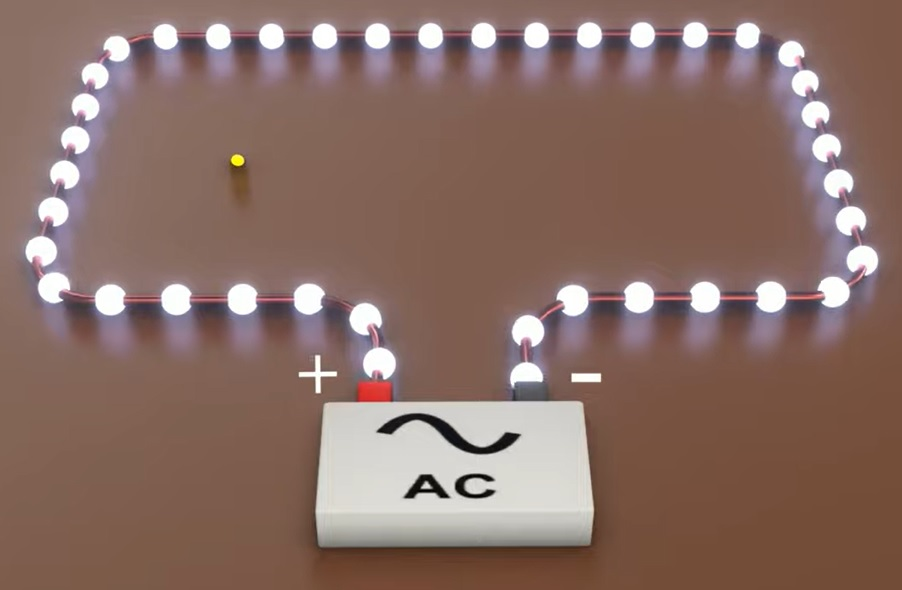
\includegraphics[width=.6\linewidth]{../figs/ac_flow.jpg}}
    \end{figure}
\end{frame}



%%%%%%%%%%%%%%%%%%

\section{Formas de onda}

\begin{frame}{Forma de onda}
    \begin{itemize}
        \item La salida de los generadores (de tensión o de corriente) es una función que puede variar con el tiempo
        \item La dependencia funcional \(u = u(t)\) o \(i = i(t)\) se denomina forma de onda

        \vspace{8mm}
        \item En este bloque temático vamos a centrarnos en \alert{formas de onda periódicas} (su valor se repite a intervalos regulares) y, en concreto, en \alert{señales senoidales}
    \end{itemize}
    \begin{center}
        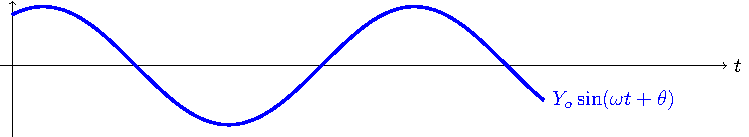
\includegraphics[width=.85\linewidth]{../figs/sin.pdf}
    \end{center}        
\end{frame}

%%%%%%%%%%%%%%%%%%

\begin{frame}{Formas de onda periódicas}    
    \vspace{-4mm}
    \begin{equation*}
        \qquad \qquad \qquad \qquad \qquad \qquad   \boxed{y(t)=y(t+T)=y(t+n\cdot T)} \quad\text{donde}\;  n\in\mathbb{Z} \;\text{(número entero)}
    \end{equation*}

    \begin{itemize}
		\item \alert{Periodo ($T$)}: intervalo de tiempo a partir del cual se repite la forma de onda [s]

        \vspace{2mm}
		\item \alert{Frecuencia ($f$)}: número de repeticiones de la onda por unidad de tiempo [Hz]
		\begin{equation*}
			f = \dfrac{1}{T}
		\end{equation*}

		\item \alert{Valor instantáneo ($y(t)$)}: valor que toma la forma de onda en un instante $t$ 

        \vspace{3mm}
		\item \alert{Valores de pico ($Y_{max}$, $Y_{min}$)}: valores máximo y mínimo que toma la forma de onda

        \vspace{-2mm}
		\begin{equation*}
			Y_{max} = \text{max}[\;f(t)\,] \qquad\quad Y_{min} = \text{min}[\;f(t)\,]
		\end{equation*}
  
        \vspace{2mm}
        Para ondas centradas ($Y_{max} \,$ = $-Y_{min}$), el valor de pico también se denomina \alert{amplitud}

        \vspace{3mm}
		\item \alert{Valor pico a pico ($Y_{PP}$)}: diferencia (en valor absoluto) entre los valores de pico considerados con signo 
  
        \vspace{-6mm}
		\begin{equation*}
			Y_{PP}=|Y_{max} - Y_{min}|
		\end{equation*}
    \end{itemize}
\end{frame}

%%%%%%%%%%%%%%%%%%

\begin{frame}{Formas de onda periódicas}
\vspace{1mm}
    \begin{itemize}
		\item Caso particular: \alert{función senoidal} (señal centrada)
    \end{itemize}

    \vspace{3mm}
    \begin{center}
        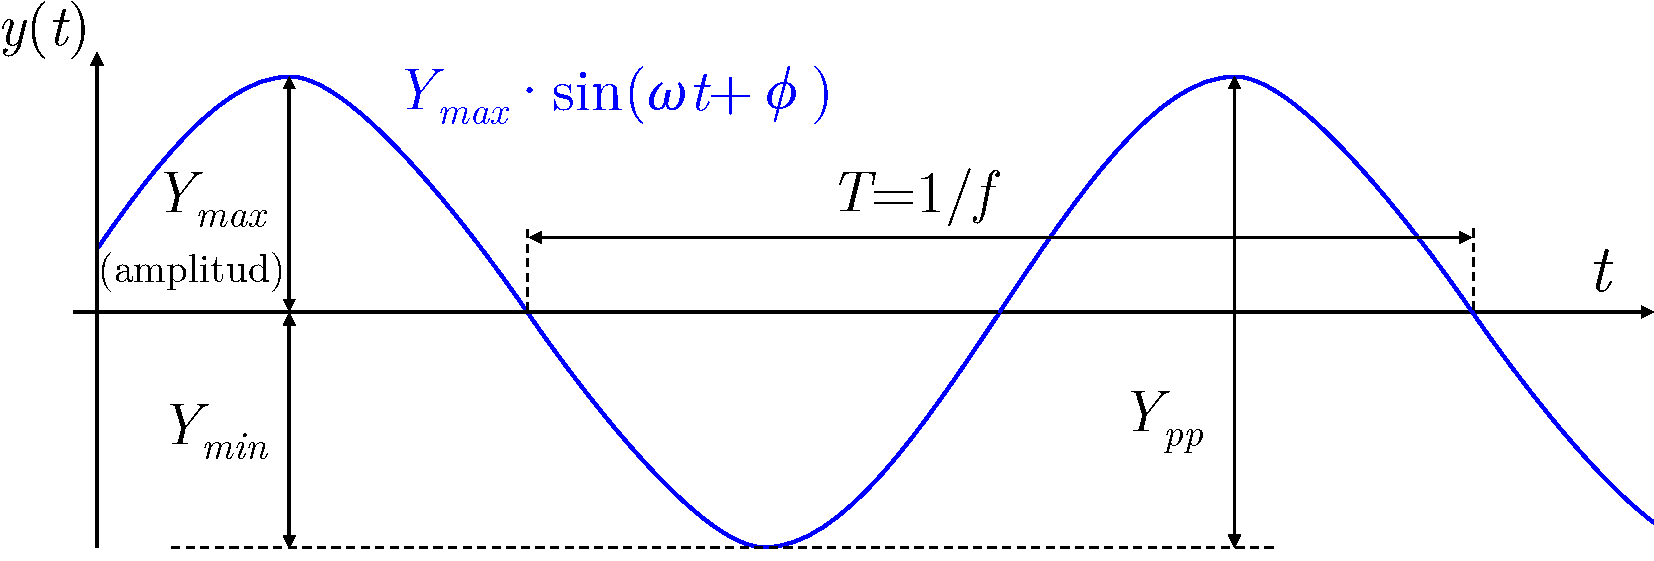
\includegraphics[width=.9\linewidth]{../figs/Senoidal_parametros.pdf}
    \end{center}   
\end{frame}

%%%%%%%%%%%%%%%%%%

\begin{frame}{Formas de onda periódicas: \hspace{3mm}valores característicos} \label{diapo:valorEficaz_definicion}
    \vspace{1mm}
    \begin{itemize}
        \item \alert{Valor medio ($Y_m$)}: media aritmética de los valores instantáneos que toma la función en un periodo (o semiperiodo, o cuarto de periodo) 
        \begin{equation*}
            \boxed{\; Y_m \; = \; \frac{1}{T}\int_{a}^{a+T}y(t)\, dt \;}
        \end{equation*}
        \item \alert{Valor eficaz ($Y_{ef}$)}: raíz cuadrada de la media de los cuadrados de los valores que toma la función en un periodo
        \begin{equation*}
            \boxed{\; Y_{ef} \, = \, \sqrt{\frac{1}{T}\cdot\int_{a}^{a+T}y^{2}(t)\, dt} \;}
        \end{equation*}
        También denominado ``valor RMS'', del inglés \textit{root mean square}

        \vspace{3mm}
        El \underline{valor eficaz es de especial interés} en teoría de circuitos para \alert{cálculos relacionados con la potencia}, como veremos más adelante
	\end{itemize}
\end{frame}

%%%%%%%%%%%%%%%%%%

\begin{frame}{Formas de onda periódicas: \hspace{3mm}valor eficaz}

    \vspace{1mm}
    \begin{itemize}
		\item Caso particular: valor eficaz de una \alert{onda senoidal}
    \end{itemize}

    \vspace{-1mm}
    \begin{center}
        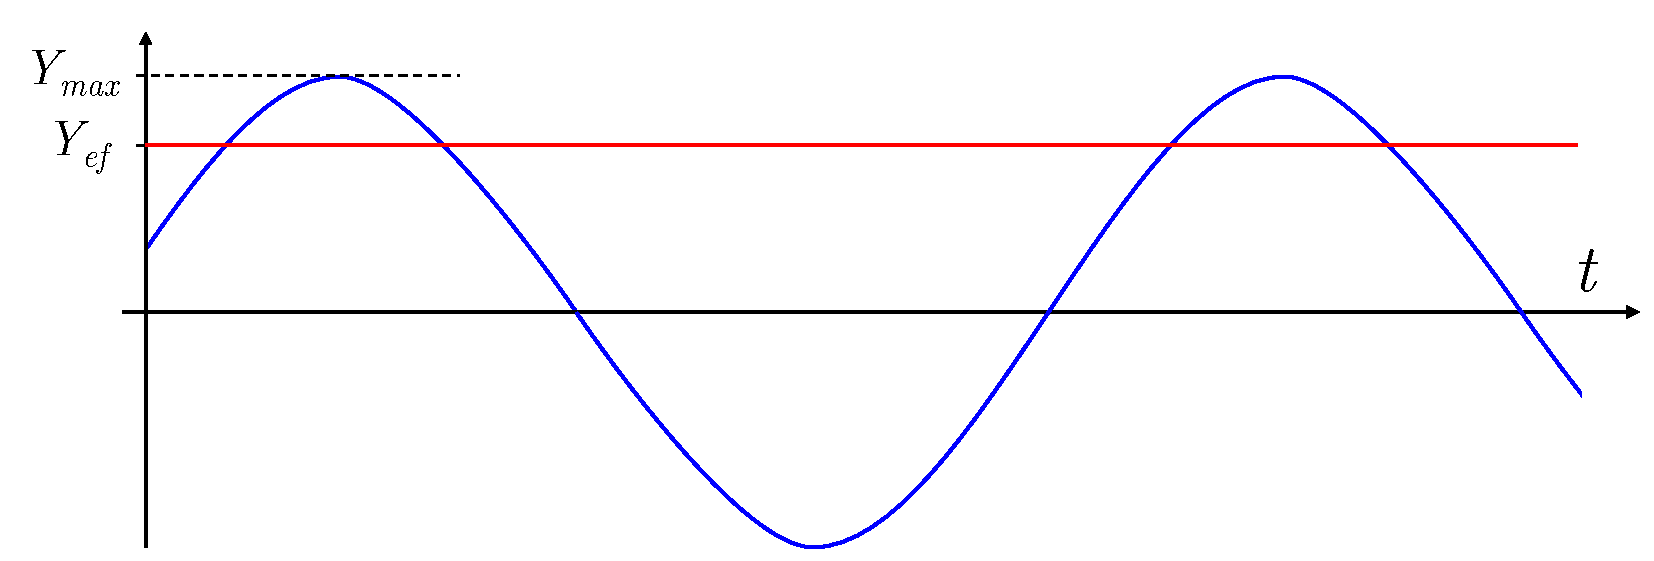
\includegraphics[width=.74\linewidth]{../figs/Senoidal_valorEficaz.pdf}
    \end{center}  

    \vspace{-2mm}
    \begin{itemize}
		\item ¿Por qué usamos el valor eficaz en corriente alterna? Porque establece un \alert{paralelismo con la corriente continua}, que nos permitirá simplificar cálculos:

        \vspace{3mm}
        El valor eficaz es \underline{igual al valor de una corriente continua constante} que, al circular por una determinada resistencia, \alert{produciría la misma disipación de potencia} que la corriente alterna que estamos considerando
    \end{itemize}

    % Veremos la demostración más adelante 
\end{frame}

%%%%%%%%%%%%%%%%%%

\section{Onda senoidal}

\begin{frame}{Onda senoidal, definición}

    \vspace{3mm}
    \begin{center}
        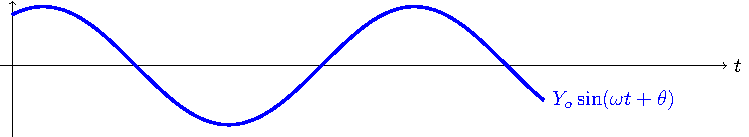
\includegraphics[width=.9\linewidth]{../figs/sin.pdf}
    \end{center}

    \vspace{-5mm}
    \[
    y(t)=Y_{o}\cdot\sin(\omega\cdot t+\theta)
    \]

    \vspace{2mm}
    
    \begin{minipage}[c]{0.45\linewidth}
        \begin{itemize}  
            \vspace{1.5mm}
            \item ${\boldsymbol{\color{blue!50!black} Y_{max} }}$ o ${\boldsymbol{\color{blue!50!black} Y_{o} }}$ : valor máximo de la onda    

            \vspace{4.5mm}
            \item ${\boldsymbol{\color{blue!50!black} T }}$ : periodo de la onda (segundos)  
        \end{itemize}
    \end{minipage}
    \hfill%
    \begin{minipage}[c]{0.45\linewidth}
        \begin{itemize}  
            \vspace{1mm}
            \item \( {\boldsymbol{\color{blue!50!black} \omega }} = \dfrac{2\pi}{T} \) : pulsación (rad/s) 
    
            \vspace{1mm}
            \item \( {\boldsymbol{\color{blue!50!black} f }} = \dfrac{\omega}{2\pi} = \dfrac{1}{T} \) : frecuencia (Hz)
        \end{itemize}
    \end{minipage}

    \begin{itemize}  
        \vspace{1.5mm}
        \item ${\boldsymbol{\color{blue!50!black} \theta }}$ : fase (radianes o grados). También suelen usarse las letras griegas $\phi$ y $\varphi$
    \end{itemize}
\end{frame}

%%%%%%%%%%%%%%%%%%

\begin{frame}{Fase}
    \begin{center}
        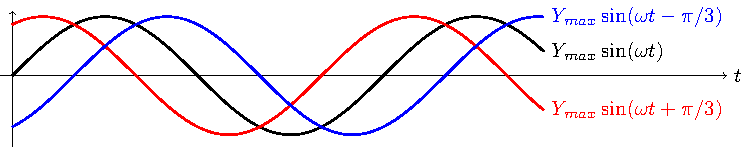
\includegraphics[width=.9\linewidth]{../figs/desfase.pdf}
    \end{center}    

    \begin{itemize}
        \item Es el argumento de la función senoidal para $t=0$        
        \vspace{2mm}
        \item Tomando una onda como referencia, si la \alert{fase de otra onda es de 0º}, está \alert{en fase} con la de referencia        
        \vspace{2mm}
        \item Si la \alert{fase es positiva}, la onda \alert{adelanta} a la referencia   

        \vspace{2mm}
        \item Si la \alert{fase es negativa}, la onda \alert{retrasa} a la referencia
    \end{itemize}
\end{frame}

%%%%%%%%%%%%%%%%%%

\begin{frame}{Señales en cuadratura}
    \begin{center}
        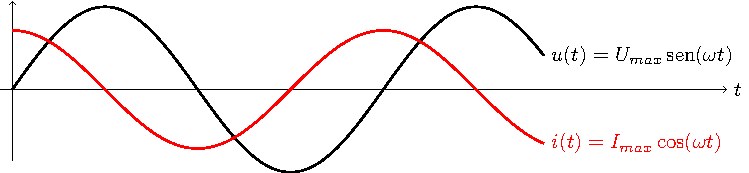
\includegraphics[width=.9\linewidth]{../figs/cuadratura.pdf}
    \end{center}
    
    \begin{itemize}
        \item Cuando el \alert{desfase entre dos señales es de 90º} (\(\theta_I - \theta_U = \pi/2\)), se dice que están en \alert{cuadratura}

        \vspace{3mm}
        \item El paso por cero de una señal coincide con el paso por el máximo/mínimo de la otra señal
    \end{itemize}
\end{frame}

%%%%%%%%%%%%%%%%%%

\begin{frame}{Valor medio y valor eficaz de una onda senoidal}
    \begin{block}{Valor medio}
        En un periodo: \[
        Y_m
        \; = \;
        \frac{1}{\boldsymbol{T}}\int_{0}^{\boldsymbol{T}}y(t)\, dt 
        \; = \;
        \frac{1}{T}\int_{0}^{T}Y_{o}\cdot\sin(\omega \cdot t +\theta)\, dt 
        \; = \;
        \boxed{\boldsymbol{0}}
        \]
        En un \href{https://raw.githubusercontent.com/ETSIDI-IE/tc/master/docs/ejercicios_clase/TC1_02_Ym_semiperiodo_senoidal_LBB.pdf}{semiperiodo positivo} ($\theta = \ang{0}$): \[
        Y_m
        \; = \;
        \frac{1}{\boldsymbol{T/2}}\int_{0}^{\boldsymbol{T/2}}Y_{max}\cdot\sin(\omega \cdot t)\, dt 
        \; = \;
        \dfrac{2\cdot Y_{max}}{\pi}
        \; \approx \; 
        0,637\cdot Y_{max}
        \]
    \end{block}
    
    \begin{block}{Valor eficaz}
        \[
        Y 
        \; = \; 
        \sqrt{\frac{1}{T}\cdot\int_{0}^{T}y^{2}(t)\, dt} 
        \; = \;
        \sqrt{\frac{1}{T}\cdot\int_{0}^{T}\left[Y_{max}\cdot\sin(\omega\cdot t+\theta)\right]^{2}dt}
        \; = \;
        \boxed{\boldsymbol{\frac{Y_{max}}{\sqrt{2}}}}
        \]
    \end{block}
\end{frame}

%%%%%%%%%%%%%%%%%%

\section{Cálculo fasorial}

\begin{frame}{Recordatorio de 1LK}
    \begin{itemize}
        \item La \alert{1LK} es el principio de \alert{conservación de la carga} aplicado a los circuitos eléctricos:
        
        \vspace{5mm}
        
        La suma de las corrientes que llegan a un nudo es igual a la suma de las que salen   

        \vspace{2mm}
        \begin{equation*}
            \large{\boxed{ \sum_{j=1}^n i_j\colorbox{yellow}{\hspace{-1mm}$(t)$\hspace{-1mm}} = 0}}
        \end{equation*}

        \vspace{2mm}
        La conservación de la carga \alert{aplica a cada instante}, luego 1LK también \alert{aplica en corriente alterna}

        \vspace{5mm}
        Por lo tanto, vamos a sumar corrientes senoidales a menudo en este tema, para lo cual será muy útil el \alert{cálculo fasorial}
        
    \end{itemize}    
\end{frame}

%%%%%%%%%%%%%%%%

\begin{frame}{Recordatorio de 2LK}
    \begin{itemize}
        \item La \alert{2LK} es el principio de \alert{conservación de la energía} aplicado a los circuitos:
        
        \vspace{5mm}
        
        La suma (con signo) de las tensiones a lo largo de un camino cerrado es cero        

        \vspace{2mm}
        \begin{equation*}
            \large{\boxed{\sum_{j=1}^m u_j\colorbox{yellow}{\hspace{-1mm}$(t)$\hspace{-1mm}} = 0}}
        \end{equation*}

        \vspace{2mm}
        La conservación de la energía \alert{aplica a cada instante} $\; \rightarrow \;$ 2LK también \alert{aplica en corriente alterna}

        \vspace{5mm}
        Vamos a sumar tensiones senoidales a menudo en este tema $\; \rightarrow \;$ será muy útil el \alert{cálculo fasorial}
    \end{itemize}    
\end{frame}

%%%%%%%%%%%%%%%%%%%%

\begin{frame}{Representación fasorial}

    \begin{center}
        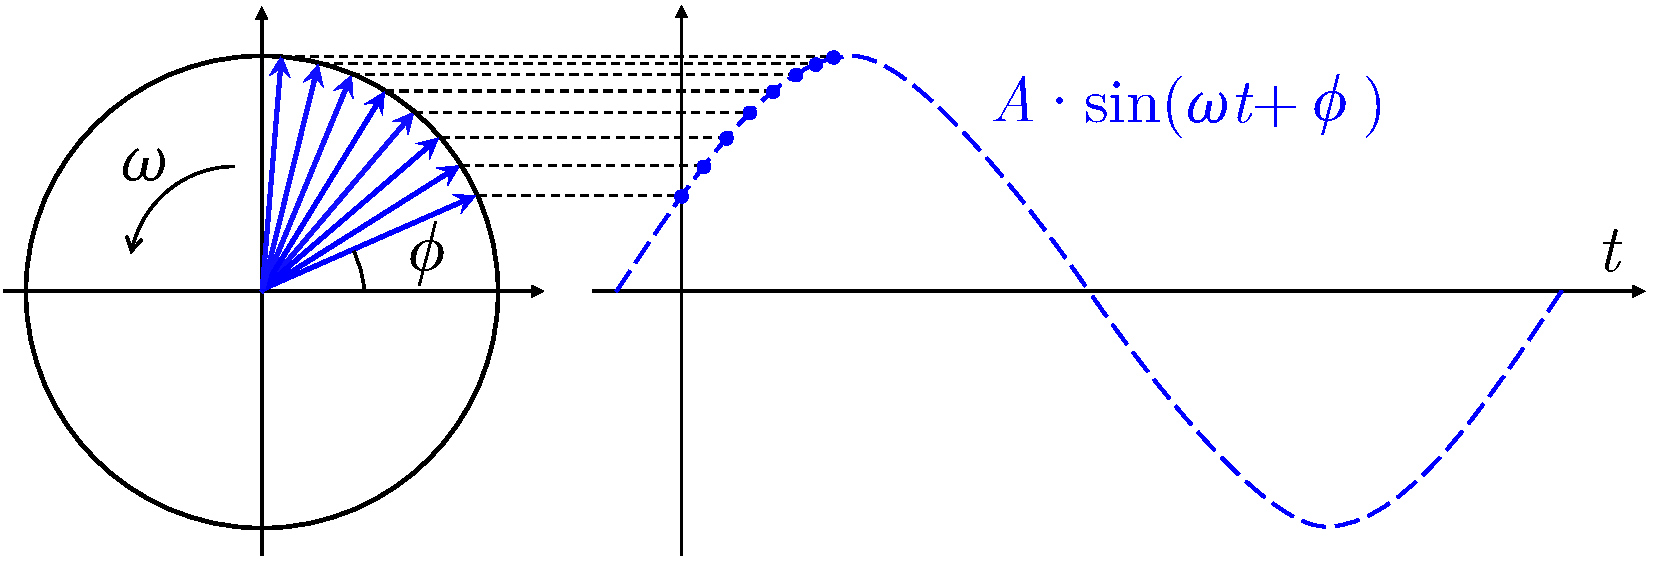
\includegraphics[height=0.45\textheight]{../figs/Fasor_rotante.pdf}
    \end{center}

    \vspace{-2mm}
    \begin{itemize}
        \item Un \alert{fasor} es un artefacto matemático \alert{útil para simplificar cálculos} con señales senoidales

        \vspace{2mm}
        \item El término ``fasor'' viene del inglés \textit{phasor}, forma corta de \textit{phase vector} (vector de fase)

        \vspace{2mm}
        \item Al \alert{rotar en sentido antihorario} con velocidad angular $\omega$, la proyección del fasor sobre el eje vertical es igual al valor de la señal senoidal en cada instante \hyperlink{diapo:gif_fasores}{.}
    \end{itemize}   

\end{frame}

%%%%%%%%%%%%%%%%%%%%

\begin{frame}{Representación fasorial}

    \begin{center}
        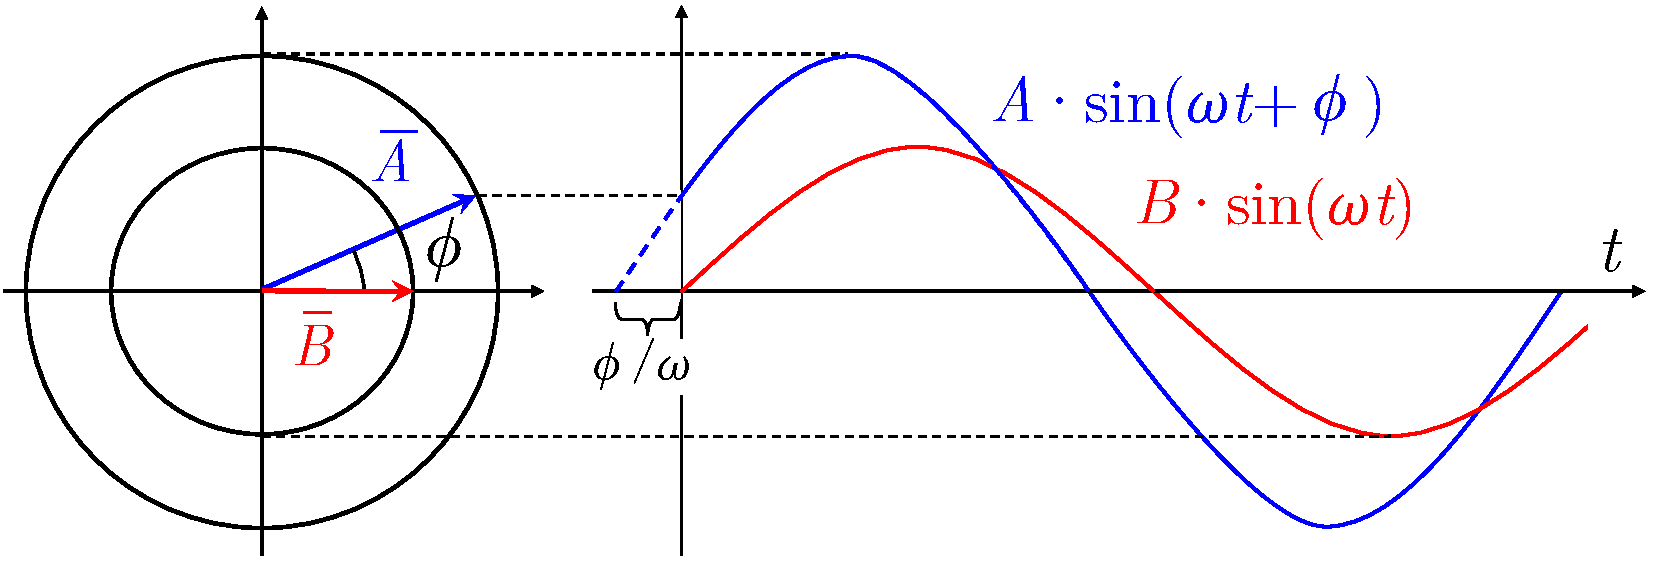
\includegraphics[height=0.45\textheight]{../figs/Fasor_definicion.pdf}
    \end{center}
    
    \begin{itemize}
        \item Una señal senoidal \alert{se representa mediante un único fasor}    

        \vspace{3mm}
        \item Para definir el fasor correspondiente a cada señal, tomamos como origen de fases una de las señales presentes en el circuito (\textit{e.g.}, la tensión en bornes de una fuente)                
    \end{itemize}   

\end{frame}

%%%%%%%%%%%%%%%%%%%%

\begin{frame}{Representación fasorial}

    \vspace{2mm}
    \begin{itemize}
        \item Un fasor se representa matemáticamente mediante un \alert{número complejo} 
        
        (\href{https://raw.githubusercontent.com/ETSIDI-IE/tc/master/docs/diapos/TC1_Trigonometria_Complejos_LBB.pdf}{repaso} de complejos y trigonometría):

        \vspace{-3mm}
        \begin{columns}
        \begin{column}{0.65\columnwidth}
        \begin{equation*}
            \overline{Y} = \underbrace{Y_{ef}\phase{\theta}}_{\substack{\text{forma} \\ \text{polar}}}
            % Para escribir el "underbrace" en varias líneas: https://tex.stackexchange.com/questions/7503/how-can-i-write-multiple-lines-in-a-subscript
            = \underbrace{Y_{ef}\cdot[\cos(\theta)+ j \cdot\sin(\theta)]}_{\text{forma binómica}}
            \overarrow[=][\downarrow]{\minibox[c]{\footnotesize fórmula  \\[-2pt] \footnotesize de Euler}}
            % Flecha, sacada de aquí: https://tex.stackexchange.com/questions/8720/overbrace-underbrace-but-with-an-arrow-instead
            % "Minibox", para poder partir el texto en 2 líneas: https://tex.stackexchange.com/questions/8680/how-can-i-insert-a-newline-in-a-framebox
            \underbrace{Y_{ef}\cdot e^{j\theta}}_{\substack{\text{forma} \\ \text{exponencial}}}
        \end{equation*}        
        \end{column}

        \begin{column}{0.35\columnwidth}
        \hspace*{-10mm}
            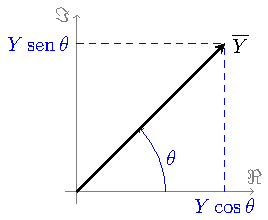
\includegraphics[height=0.5\textheight]{../figs/fasor.pdf}
        
        \end{column}        
        \end{columns}

        \vspace*{3mm}
        Usamos \alert{\textit{j} para la constante imaginaria}, en lugar de \textit{i}, ya que en el análisis de circuitos \textit{i} se usa para intensidad
    \end{itemize}    
    
    \begin{itemize}
        \item El \alert{argumento} del fasor es la \alert{fase} de la onda. El \alert{módulo} es el \alert{\underline{valor eficaz}} de la onda, \textcolor{red}{NO su amplitud} 
    \end{itemize}

\end{frame}

%%%%%%%%%%%%%%%%%%%

\begin{frame}{Representación fasorial}  

    \vspace{2mm}
    \begin{itemize}
        \item El \alert{argumento} del fasor es la \alert{fase} de la onda. El \alert{módulo} es el \alert{\underline{valor eficaz}} de la onda, \textcolor{red}{NO su amplitud} 

        \vspace*{3mm}
        Se toma el valor eficaz por \alert{conveniencia a la hora de calcular la potencia producida/ consumida} en circuitos de corriente alterna, directamente operando con fasores

        \vspace*{4mm}
        \fbox{ \begin{minipage}{0.97\linewidth} 
        \alert{\textcolor{red}{Nota}}: en varios gráficos de estas diapositivas, el módulo de los fasores corresponde a la amplitud de la onda, y no a su valor eficaz         
        
        Esto se debe simplemente a claridad en la representación gráfica
        \end{minipage} }
    \end{itemize}
    
    \begin{center}
        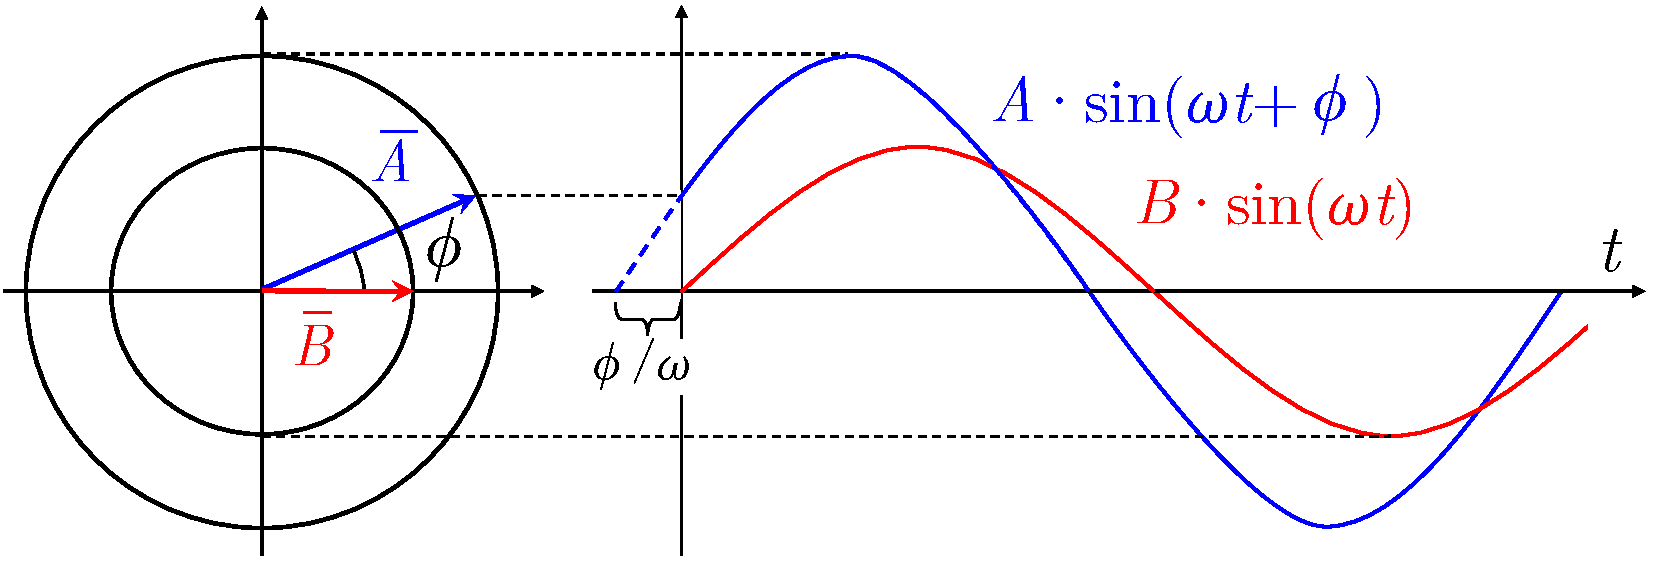
\includegraphics[height=0.35\textheight]{../figs/Fasor_definicion.pdf}
    \end{center}
\end{frame}

%%%%%%%%%%%%%%%%%%%

\begin{frame}{Representación fasorial}  

    \vspace{2mm}
    \begin{itemize}       
        \item Los fasores \alert{representan las relaciones entre los valores eficaces y las fases} de las distintas señales presentes en el circuito, siempre asumiendo una frecuencia determinada 

        \vspace{3mm}
        \item Por lo tanto, las operaciones con fasores \alert{solo son válidas entre \underline{señales de la misma} \underline{frecuencia}} \hyperlink{diapo:fasores_distintaFrecuencia}{.}
    \end{itemize}
    
    \begin{center}
        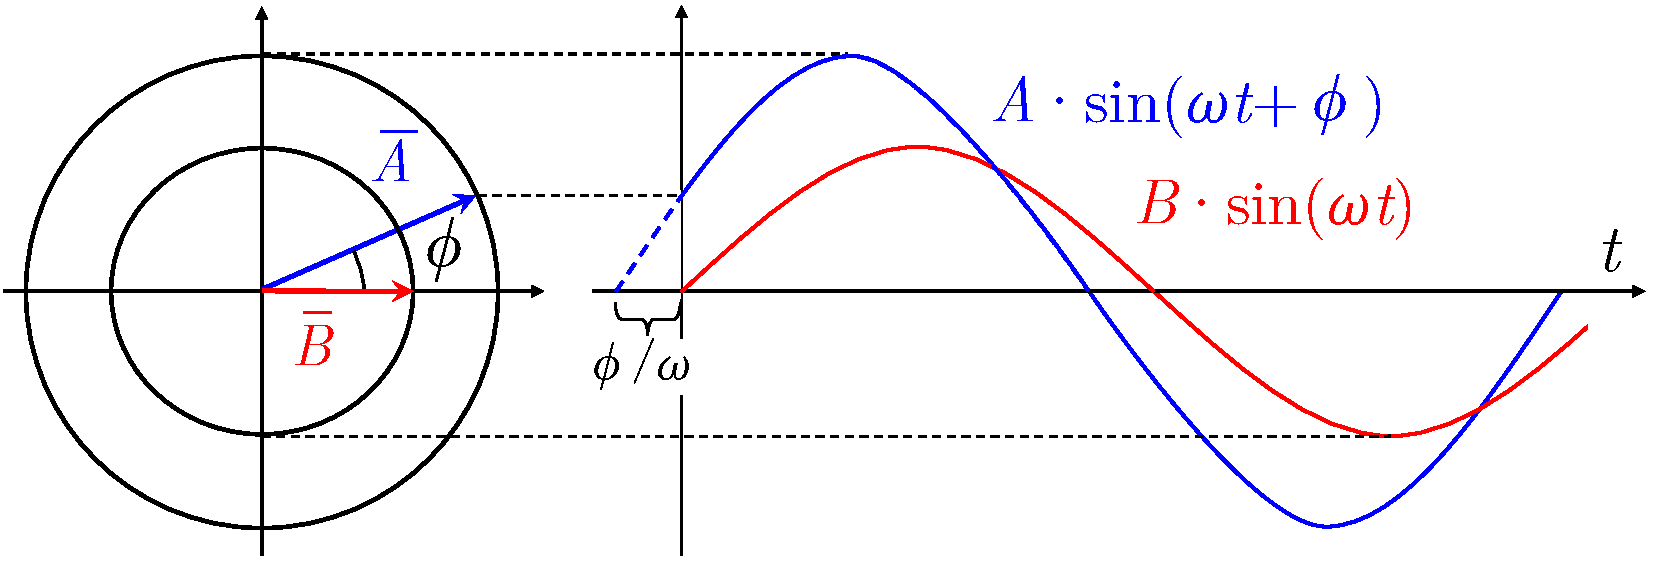
\includegraphics[height=0.45\textheight]{../figs/Fasor_definicion.pdf}
    \end{center}
    %\alert{\textcolor{red}{Nota:}} en el diagrama se usa el módulo de los fasores igual a la amplitud de onda y no al  valor eficaz, simplemente por claridad gráfica. 
    
\end{frame}

%%%%%%%%%%%%%%%%%%

\begin{frame}{Cálculo fasorial: \hspace{3mm}propiedades de la función senoidal} 

    \vspace{3mm}
    Las razones por las que podemos usar cálculo fasorial para \alert{simplificar operaciones entre señales senoidales} son dos propiedades importantes de la función senoidal:

    \begin{itemize}       
        \item \fbox{ \begin{minipage}{0.97\linewidth} 
        $ \vphantom{\dfrac{1}{1}} \qquad\qquad\quad A_1 \cdot \sin(\omega t + \theta_1) 
        \; + \;
        A_2 \cdot \sin(\omega t + \theta_2)
        \; = \;
        A_3 \cdot \sin(\omega t + \theta_3)
        $
        %La \alert{suma de dos senoidales} de igual frecuencia (independientemente de sus fases o amplitudes) da como resultado otra \alert{senoidal de la misma frecuencia}
        \end{minipage} } 

        \vspace*{3mm}
        Para sumar señales senoidales, podemos simplemente \alert{sumar sus fasores correspondientes} (recuerda que 1LK y 2LK implican sumas)
        \vspace*{5mm}

        \item \fbox{ \begin{minipage}{0.97\linewidth} 
        $ \vphantom{\dfrac{\frac{\int}{1}}{frac{1}{1}}} 
        \dfrac{d^n \sin(\omega t + \theta_1)}{dt^n} = C_2 \sin(\omega t + \theta_2) \;\; ,
        \;\;\;\,
        \bigintsss \hspace{-1mm} 
        \cdot\hspace{-1mm} \cdot \hspace{-1mm}\cdot 
        \hspace{-1mm}\bigintsss \hspace{-1mm}\sin(\omega t + \theta_1) \,dt
        \cdot\hspace{-1mm} \cdot \hspace{-1mm}\cdot 
        dt = C_3 \sin(\omega t + \theta_3) + k
        $ % "\bigintsss" from here, https://tex.stackexchange.com/questions/39181/big-integral-sign
        %
        %Las sucesivas \alert{derivadas e integrales de una senoidal} son también funciones \alert{senoidales de la misma frecuencia}
        \end{minipage} } 

        \vspace*{3mm}
        Las \alert{tensiones y corrientes en bobinas y condensadores} (cuyas ecuaciones de definición contienen derivadas e integrales de estas magnitudes), \alert{pueden expresarse mediante fasores}       
    \end{itemize}  
\end{frame}

%%%%%%%%%%%%%%%%%%%

\begin{frame}{Operaciones con fasores} \label{diapo:gif_fasores} 
    
    \vspace{3mm}
    Suma gráfica de dos fasores $\overline{Y}_1$ e $\overline{Y}_2$, y sus correspondientes señales temporales:
    
    (\alert{clica en la imagen})

    % Ejemplo gráfico de "suma de varias senoidales de igual frecuencia da como resultado otra senoidal de esa misma frecuencia"
    \begin{center}
    \animategraphics[loop,width=12cm]{10}{../figs/gifs/Sumafasores-}{0}{47}
    \end{center}
    % Info para insertar .gif: https://latex-beamer.com/tutorials/gif-latex-beamer/    
    % Esta info también está en "figs\insert_GIF_Beamer.pdf"
\end{frame}

%%%%%%%%%%%%%%%%%%

\begin{frame}{Operaciones con fasores}
    \begin{itemize}       
        \item Un fasor \alert{captura la información clave de una onda senoidal} para los propósitos del análisis de circuitos: su \underline{valor eficaz} y su \underline{fase} 

        \vspace{1mm}
        \item Nos permite \alert{operar con ondas senoidales como si fueran vectores/números complejos}
    \end{itemize}     
    \vspace*{-7mm}
    \begin{align*}
        \overline{Y}_1 & \; = \; 
        \overbrace{Y_{ef_1}\,\cos(\theta_1)}^{a_1}+\,\mathrm{j}\,\overbrace{Y_{ef_1}\;\sin(\theta_1)}^{b_1} 
        \; = \; 
        Y_{ef_1}\phase{\theta_1}\\
        \overline{Y}_2 & \; = \; \underbrace{Y_{ef_2}\,\cos(\theta_2)}_{a_2}+\;\mathrm{j}\,\underbrace{Y_{ef_2}\,\sin(\theta_2)}_{b_2}
        \; = \; 
        Y_{ef_2}\phase{\theta_2}
    \end{align*}
    
    \vspace*{-6mm}
    Forma binómica:

    \vspace*{-1mm}
    \begin{itemize}
        \item Suma: $\quad \overline{Y}_1+\overline{Y}_2 \; = \; (a_1+a_2)+\mathrm{j}\,(b_1+b_2)$

        \vspace{2mm}
        \item Resta: $\quad \overline{Y}_1-\overline{Y}_2 \; = \; (a_1-a_2)+\mathrm{j}\,(b_1-b_2)$
    \end{itemize}
    Forma polar:
    \begin{itemize}
        \item Multiplicación: $\quad \overline{Y}_1\cdot \overline{Y}_2 \; = \; (Y_{ef_1}\cdot Y_{ef_2})\phase{\theta_1+\theta_2}$
        \item División: $\quad \dfrac{\overline{Y}_1}{\overline{Y}_2} \; = \; \dfrac{Y_{ef_1}}{Y_{ef_2}}\phase{\theta_1-\theta_2}$
    \end{itemize}    
\end{frame}

%%%%%%%%%%%%%%%%%%%%%%%

\begin{frame}{Interludio: \hspace{6mm}\textit{Alternating Current} \hspace{1mm}\faBolt \hspace{1mm} \textit{Direct Current}}    
		\centering 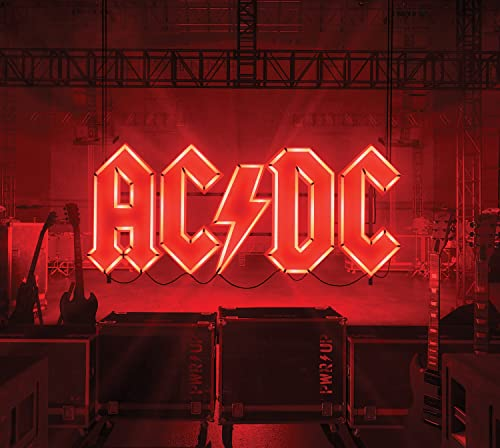
\includegraphics[width=0.4\linewidth]{../figs/AC_DC_grupo.jpg}
\end{frame}

%%%%%%%%%%%%%%%%%%

\section{Respuesta de elementos pasivos a excitación senoidal}

\begin{frame}{Impedancia: \hspace{3mm}relación entre fasores de tensión y corriente}
    \vspace{2mm}
    \begin{center}
        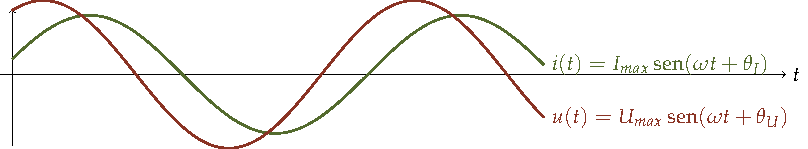
\includegraphics[width=.9\linewidth]{../figs/ondasTensionCorriente.pdf}
    \end{center}

    \vspace{-7mm}
    \begin{columns}
    \begin{column}{0.5\columnwidth}

        \vspace{3mm} 
        \begin{align*}
          \qquad\qquad\quad \overline{U} &= \overline{Z} \cdot \overline{I} \quad \text{(equiv. a \alert{ley de Ohm})}\\[10pt] 
          \qquad\qquad\quad \overline{Z} &= \frac{\overline{U}}{\overline{I}}
        \end{align*}

        \vspace{-6mm} 
        \[
        \qquad \boxed{\quad \overline{Z} = \frac{U}{I}\phase{\theta_U - \theta_I} \quad \Rightarrow \quad
            \begin{cases}
              Z = \dfrac{U}{I}\\[8pt]
              \theta = \theta_U - \theta_I
            \end{cases}}
        \]
    \end{column}    
    \begin{column}{0.5\columnwidth}
        \begin{center}
            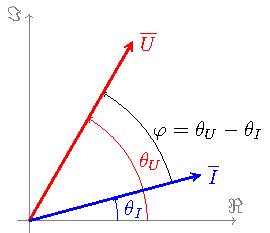
\includegraphics[height=0.6\textheight]{../figs/fasorTensionCorriente.pdf}
        \end{center}
    \end{column}
    \end{columns}
\end{frame}

%%%%%%%%%%%%%%%%%%

\begin{frame}{Impedancia genérica}
    \vspace{3mm}
    \[
    \overline{Z} \;\; = \;\; Z\cdot\cos(\theta) \; + \; \mathrm{j}\,Z\cdot\sin(\theta) \;\; = \hspace{-2mm} \underbrace{R}_\text{resistencia}\hspace{-1mm} + \;\; \mathrm{j} \hspace{-2mm}\underbrace{X}_\text{reactancia}
    \]
    
    \vspace{-3mm}

    \hspace{30mm}
    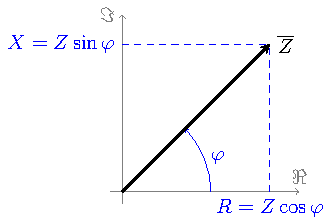
\includegraphics[height=0.65\textheight]{../figs/fasorImpedancia.pdf}

\end{frame}

%%%%%%%%%%%%%%%%%%%%%%%%

\begin{frame}{Circuito resistivo}
    \vspace{1mm}
    Un circuito resistivo no introduce desfase entre señales (\alert{tensión y corriente en fase})
    
    \begin{center}
        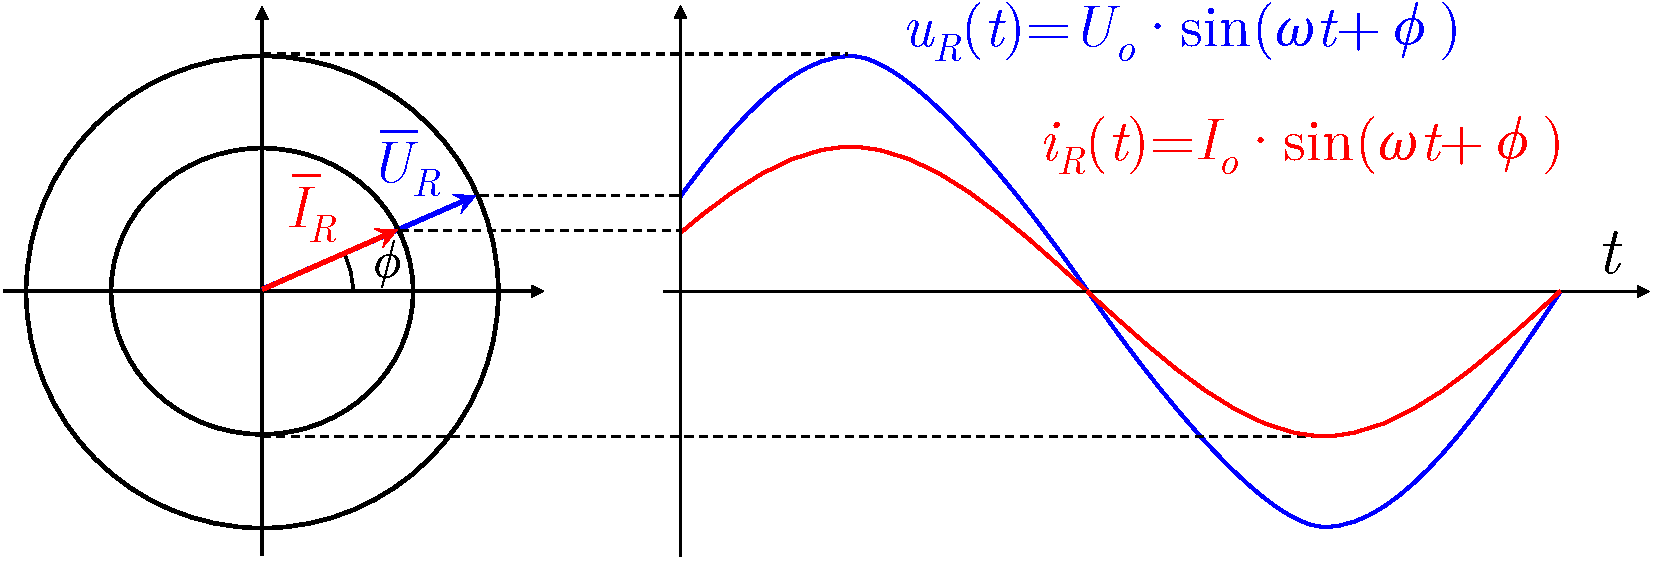
\includegraphics[height=0.45\textheight]{../figs/Fasores_resistencia.pdf}
    \end{center}

    \vspace{-4mm}
    \[
        i(t) = \boldsymbol{\color{blue!50!black} I \sqrt2} \cdot \sin(\omega t + \boldsymbol{\color{blue!50!black} \theta_I})
    \]
    \vspace*{-8mm}
    \[
        u(t) \overarrow[=][\downarrow]{\footnotesize ley de Ohm\vspace*{-1mm}}
             R \cdot i(t)
             = \boldsymbol{\color{blue!50!black} R \cdot I \sqrt2} \cdot \sin(\omega t + \boldsymbol{\color{blue!50!black}  \theta_I})
             = \boldsymbol{\color{blue!50!black}  U \sqrt2} \cdot \sin(\omega t + \boldsymbol{\color{blue!50!black}  \theta_I})
    \]

    \vspace{-2mm}
    
    \noindent\rule{\textwidth}{0.5pt}

    \vspace{-2mm}

    \begin{center}
        (a partir de ahora, la notación $U$ e $I$ se refiere directamente a \alert{valores eficaces})
    \end{center}
\end{frame}

%%%%%%%%%%%%%%%%%%%%%%%%%%%

\begin{frame}{Circuito resistivo}
    \vspace{2mm}
    Un circuito resistivo no introduce desfase entre señales (\alert{tensión y corriente en fase})

    \vspace{1mm}
    \begin{center}
        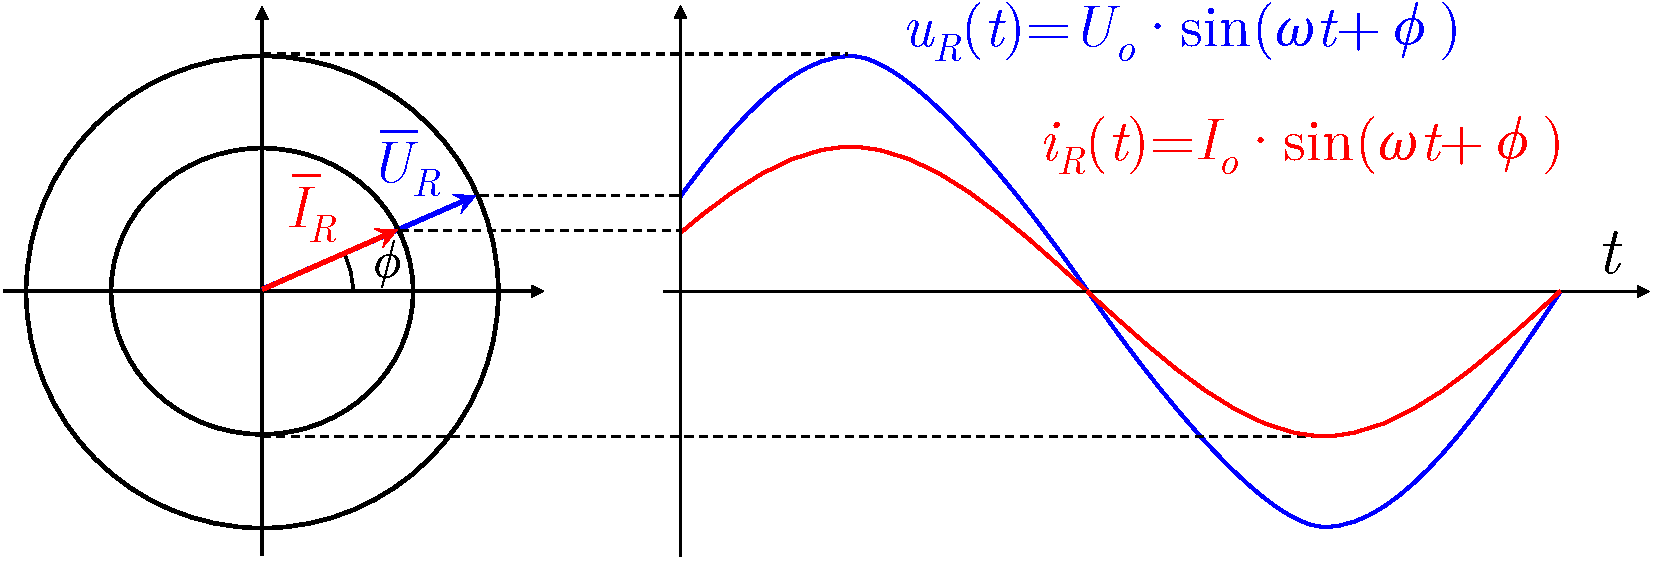
\includegraphics[height=0.4\textheight]{../figs/Fasores_resistencia.pdf}
    \end{center}

    \vspace{-2mm}
    \begin{columns}
    \begin{column}{0.3\columnwidth}
        \begin{align*}
          Z &= \frac{U}{I} = R\\
          \theta &= \theta_U - \theta_I = \ang{0}\\
          \Aboxed{\;\; \overline{Z}_R &= R \phase{\ang{0}} \;\; }
        \end{align*}
    \end{column}
    
    \begin{column}{0.35\columnwidth}
        \begin{center}
            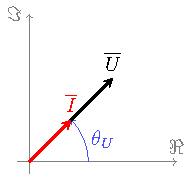
\includegraphics[height=0.35\textheight]{../figs/fasorResistencia_VI.pdf}
        \end{center}
    \end{column}    
    
    \begin{column}{0.35\columnwidth}
        \begin{center}
            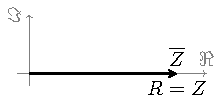
\includegraphics[height=0.25\textheight]{../figs/fasorResistencia.pdf}
        \end{center}
    \end{column}
    \end{columns}
\end{frame}

%%%%%%%%%%%%%%%%%%%%%%%

\begin{frame}{Carga y descarga de una bobina}  

\vspace{2mm}
    \begin{itemize}
        \item La bobina \alert{almacena energía magnética} cuando circula por ella una corriente
        \[
            E_L = \tfrac{1}{2}\cdot L \cdot i_L^2(t)
        \]
        
        %\vspace{-2mm}
        Cuando el módulo de la corriente que circula por la bobina disminuye, \alert{devuelve su energía almacenada} al circuito \hspace{15mm}(\alert{clica en la imagen})        
    \end{itemize}

    % https://www.youtube.com/watch?v=d73e3QiMdSU
    \begin{center}
        \animategraphics[loop,width=9.4cm]{10}{../figs/gifs/inductance/}{1}{81}
    \end{center}
    % Info para insertar .gif: https://latex-beamer.com/tutorials/gif-latex-beamer/  
    % Esta info también está en "figs\insert_GIF_Beamer.pdf"
\end{frame}

%%%%%%%%%%%%%%%%%%%%%%%%%%%

\begin{frame}{Circuito inductivo puro}
    \vspace{2mm}
    Un circuito inductivo puro genera \alert{señales en cuadratura} y \underline{\alert{retrasa la corriente}} \href{https://raw.githubusercontent.com/ETSIDI-IE/tc/master/docs/diapos/TC1_Trigonometria_Complejos_LBB.pdf}{.}

    \vspace{1mm}
    \begin{center}
        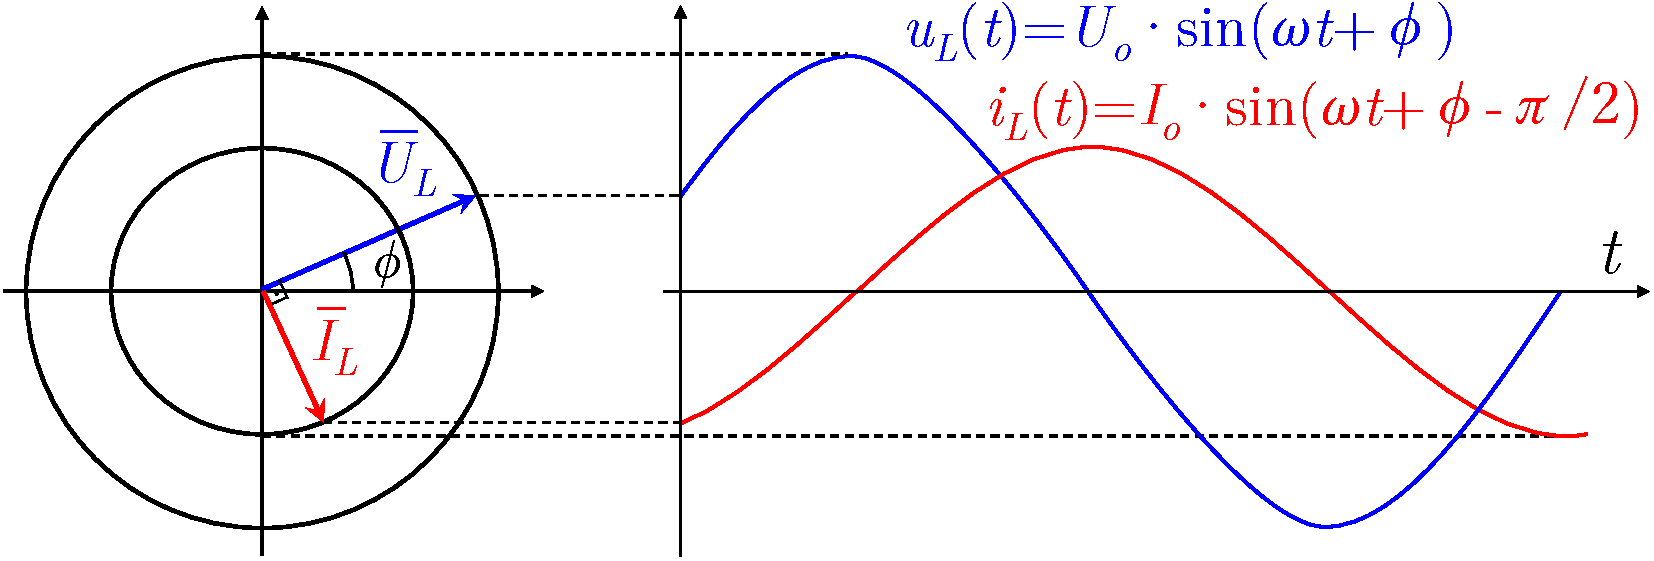
\includegraphics[height=0.48\textheight]{../figs/Fasores_inductancia.pdf}
    \end{center}

    \vspace{-8mm}
    \[
        \qquad\qquad\qquad\qquad\qquad\qquad\; i(t) = \boldsymbol{\color{blue!50!black} I\,\sqrt{2} } \cdot \sin(\omega t + \theta_I)
        \qquad
        \boxed{\text{ \begin{minipage}{0.35\linewidth} \footnotesize La bobina se carga cuando \\$\diff{|i_L|}{t}>0$, y descarga cuando $\diff{|i_L|}{t}<0$ \end{minipage} } }
    \]
    \vspace*{-11mm}
    \[
      u(t) \overarrow[=][\downarrow]{\minibox[c]{\footnotesize ley de \\[-2pt] \footnotesize Faraday}}
           L \cdot \frac{d i(t)}{dt} 
           =
           \boldsymbol{\color{blue!50!black}\omega L \cdot I\,\sqrt{2}} \cdot \cos(\omega t + \theta_I) 
           = {\boldsymbol{\color{blue!50!black}U\,\sqrt{2}}} \cdot \sin(\omega t + \theta_I \boldsymbol{\color{blue!50!black} +\pi/2})
    \]
\end{frame}

%%%%%%%%%%%%%%%%%%

\begin{frame}{Circuito inductivo puro}

    \vspace{2mm}
    Un circuito inductivo puro genera \alert{señales en cuadratura} y \underline{\alert{retrasa la corriente}}
    
    \begin{center}
        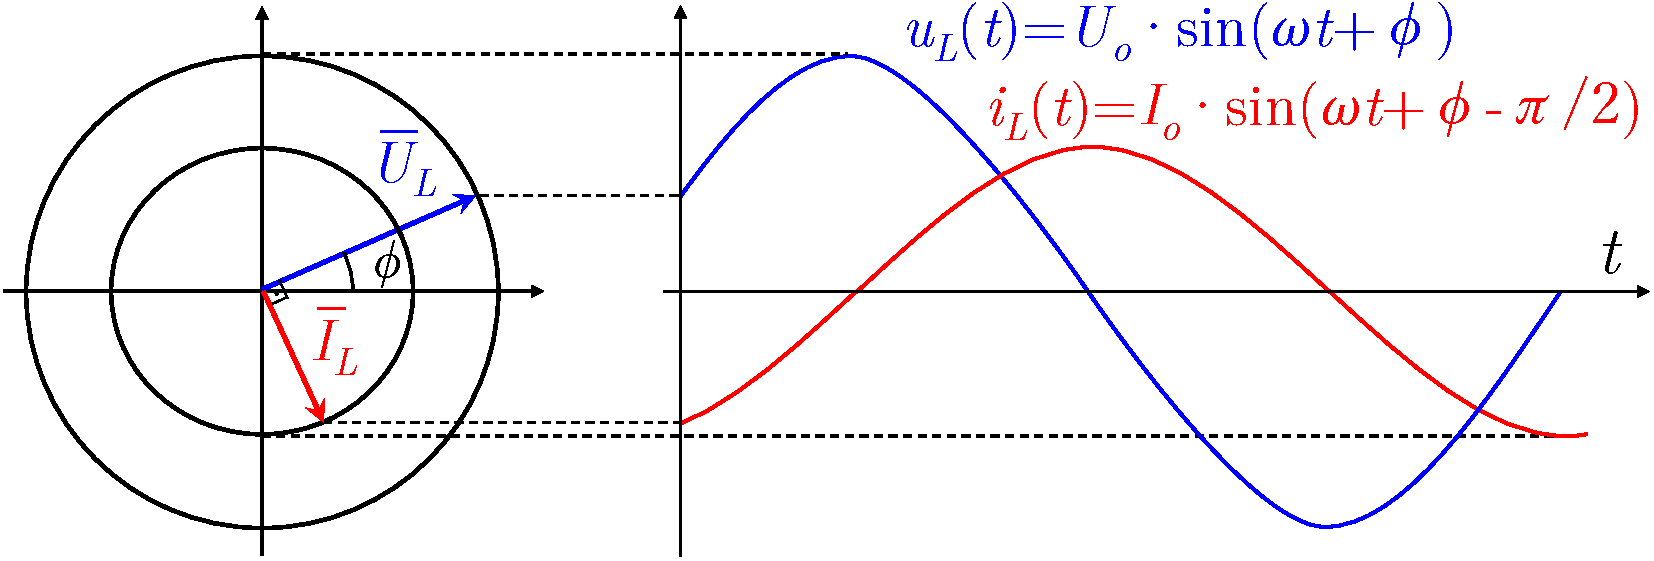
\includegraphics[height=0.37\textheight]{../figs/Fasores_inductancia.pdf}
    \end{center}  

    \vspace{-2mm}
    \begin{columns}
    \begin{column}{0.3\columnwidth}
    
        \vspace{-4mm}
        \begin{align*}
          Z &= \frac{U}{I} = \omega L\\
          \theta &= \theta_U - \theta_I = \frac{\pi}{2}\\[3pt]
          \Aboxed{\;\; \overline{Z}_L &= j\omega L = \omega L \phase{\ang{90}} \;\;}
        \end{align*}
    \end{column}        
    \begin{column}{0.4\columnwidth}
        \begin{center}
            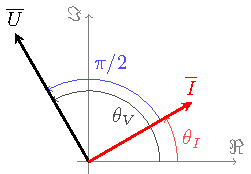
\includegraphics[height=0.4\textheight]{../figs/fasorInductancia_VI.pdf}
        \end{center}
    \end{column}  
    \begin{column}{0.3\columnwidth}
        \begin{center}
            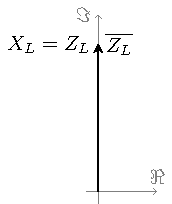
\includegraphics[height=0.4\textheight]{../figs/fasorInductancia.pdf}
        \end{center}
    \end{column}
    \end{columns}
\end{frame}

%%%%%%%%%%%%%%%%%%%%%%%

\begin{frame}{Carga y descarga de un condensador}  

\vspace{2mm}
    \begin{itemize}
        \item Si se excita un condensador con pulsos rectangulares de tensión, se \alert{almacena energía eléctrica, que luego se devuelve al circuito} en los semiciclos sin excitación
        \vspace{0.5mm}
    \end{itemize}
    
    \hspace{20mm}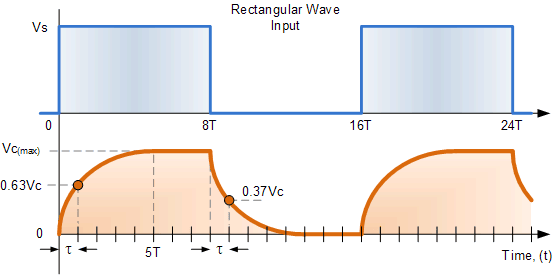
\includegraphics[width=0.62\linewidth]{../figs/charging_discharging_capacitor_pulses.png} 
    
    \vspace{-30mm}
    \[
        \qquad\qquad\qquad\qquad\qquad\qquad\qquad\qquad\qquad\qquad\qquad\qquad\qquad\qquad\quad\boxed{\text{ \begin{minipage}{0.12\linewidth} \footnotesize Energía \\ almacenada: \\[5pt] $\frac{1}{2}\cdot C\cdot u_C^2(t)$ \end{minipage} } }
    \]

    \vspace{6mm}
    \begin{itemize}
      \item Con \alert{excitación alterna senoidal}, el condensador también se carga y descarga

      \vspace{1mm}
        \begin{itemize}
            \item {\normalsize Sin embargo, la tensión en el condensador nunca llega a estabilizarse, porque la excitación senoidal cambia todo el rato \hspace{3mm}(siguiente diapositiva)}
        \end{itemize}
    \end{itemize}
\end{frame}

%%%%%%%%%%%%%%%%%%%%

\begin{frame}{Circuito capacitivo puro}

    \vspace{2mm}
    Un circuito capacitivo puro genera \alert{señales en cuadratura} y \underline{\alert{adelanta la corriente}} \href{https://raw.githubusercontent.com/ETSIDI-IE/tc/master/docs/diapos/TC1_Trigonometria_Complejos_LBB.pdf}{.}

    \vspace{1mm}
    \begin{center}
            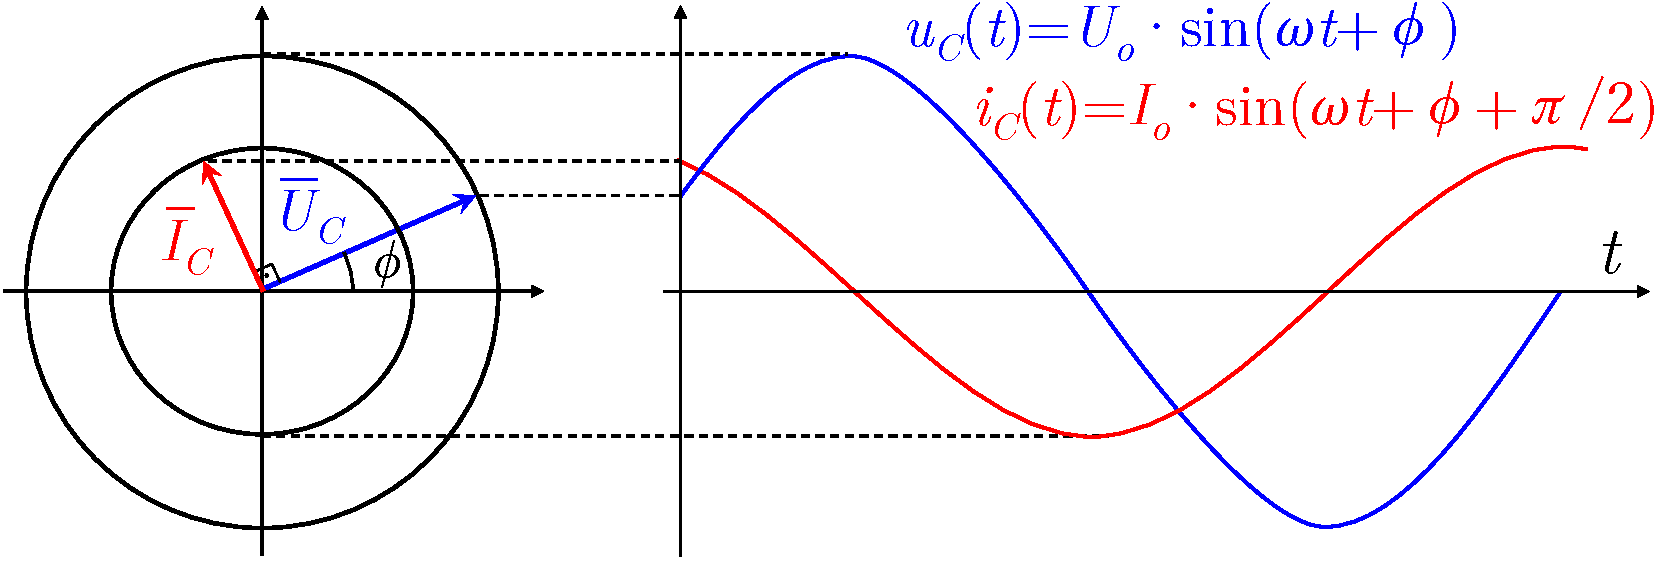
\includegraphics[height=0.48\textheight]{../figs/Fasores_condensador.pdf}
        \end{center}

    \vspace{-8mm}
    \[
        \qquad\qquad\qquad\qquad\qquad\qquad i(t) = \boldsymbol{\color{blue!50!black} I\,\sqrt{2} } \cdot \sin(\omega t + \theta_I)
        \qquad
        \boxed{\text{ \begin{minipage}{0.37\linewidth} \footnotesize El condensador se carga cuando \\$\diff{|u_C|}{t}>0$, y descarga cuando $\diff{|u_C|}{t}<0$ \end{minipage} } }
    \]
    \vspace*{-11mm}
    \[
         u(t) \overarrow[=][\downarrow]{\minibox[c]{\footnotesize definición \\[-2pt] \footnotesize de condensador}}         
         \dfrac{1}{C}\cdot\int_{-\infty}^{t} i(\tau)\cdot d\tau
         = 
         \boldsymbol{\color{blue!50!black} \dfrac{I}{\omega\,C}\sqrt{2}}\cdot [-\cos (\omega t+ \theta_I)] 
         = 
         \boldsymbol{\color{blue!50!black} U\sqrt{2}}\cdot\sin \left(\omega t+ \theta_I \boldsymbol{\color{blue!50!black} -\pi/2}\right)
         % Nota: LA INTEGRAL NO ES DIVERGENTE, porque el área bajo los semiperiodos positivos se cancela con la de los negativos desde -inf hasta el último periodo que todavía no ha terminado en el instante "t", así que la integral se puede calcular únicamente en esta última "porción" de periodo
    \]
\end{frame}

%%%%%%%%%%%%%%%%

\begin{frame}{Circuito capacitivo puro}
    \vspace{2mm}
    Un circuito capacitivo puro genera \alert{señales en cuadratura} y \underline{\alert{adelanta la corriente}}
    
    \begin{center}
            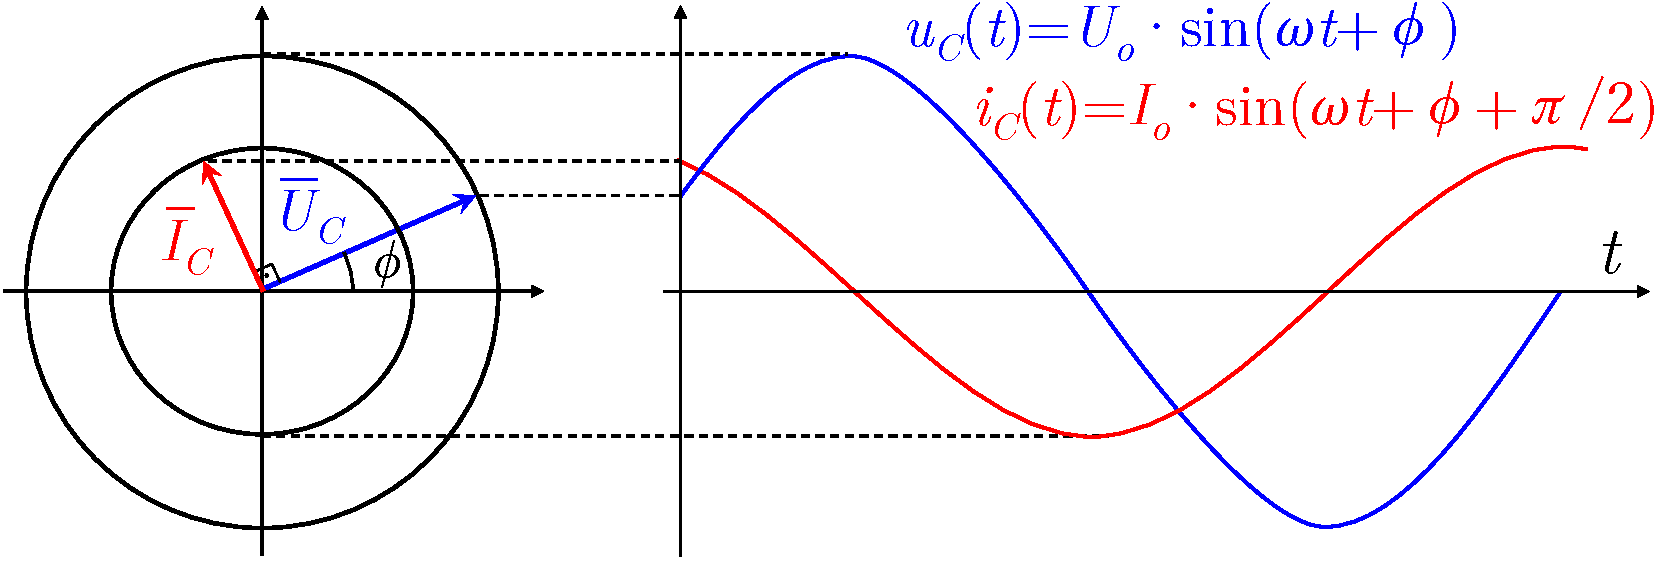
\includegraphics[height=0.37\textheight]{../figs/Fasores_condensador.pdf}
        \end{center} 

    \vspace{-2mm}
    \begin{columns}
    \begin{column}{0.3\columnwidth}

        \vspace{-4mm}
        \begin{align*}
          Z &= \frac{U}{I} = \frac{1}{\omega C}\\
          \theta &= \theta_U - \theta_I = - \frac{\pi}{2}\\[3pt]
          \Aboxed{\;\; \overline{Z}_C &= \frac{1}{j\omega C} = \frac{1}{\omega C}\phase{\ang{-90}} \;\;}
        \end{align*}
    \end{column}
    \begin{column}{0.4\columnwidth}
        \begin{center}
            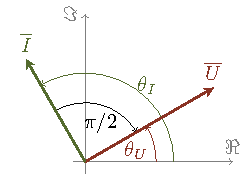
\includegraphics[height=0.4\textheight]{../figs/fasorCondensador_VI.pdf}
        \end{center}
    \end{column}  
    \begin{column}{0.3\columnwidth}
        \begin{center}
            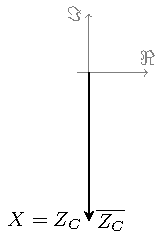
\includegraphics[height=0.4\textheight]{../figs/fasorCondensador.pdf}
        \end{center}
    \end{column}
    \end{columns}
\end{frame}

%%%%%%%%%%%%%%%%%%%%%%%

\begin{frame}{Resumen}
\vspace{7mm}
\[
  \begin{array}{lccc}
    \text{Elemento} & \text{Impedancia} & \text{Módulo} & \text{Ángulo}\\
    \hline\\[-8pt]
    \text{Resistencia} & R & R & \ang{0}\\[3pt]
    \text{Bobina ideal} & j \omega L & \omega L & \ang{90}\\[3pt]
     \text{Condensador} & 1/(j \omega C) & 1/(\omega C) & \ang{-90}\\
  \end{array}
\]

\vspace*{12mm}
\begin{itemize}
    \item La impedancia de una \alert{bobina ideal} $\, X_L=\omega L \,$ se denomina ``reactancia inductiva''

    \vspace{3mm}
    \item La impedancia de un \alert{condensador} $\, X_C=\dfrac{1}{\omega C} \,$ se denomina ``reactancia capacitiva''
\end{itemize}

\end{frame}

%%%%%%%%%%%%%%%

\begin{frame}{Interludio: \hspace{3mm}película relacionada con la asignatura}
    \begin{center}
    \href{https://www.youtube.com/watch?v=2FTxKFsWz60}{La guerra de las corrientes}, 2017
    
    
\includegraphics[width=0.38\linewidth]{../figs/War_of_currents.jpg}
    \end{center}
\end{frame}

%%%%%%%%%%%%%%%

\begin{frame}{Circuito RL \hspace{3mm}(inductivo con pérdidas)}    
    %\begin{center}
    %    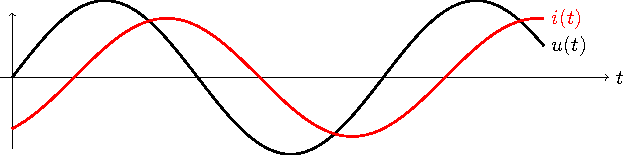
\includegraphics[height=0.25\textheight]{../figs/inductivo.pdf}
    %\end{center}

    \vspace{3mm}
    \alert{Recordatorio}: por elementos asociados en \alert{serie}, circula la \alert{misma corriente}

    \vspace{1mm}
    \begin{columns}
    \begin{column}{0.5\columnwidth}
    
        \vspace{-3mm}
        \begin{center}
            \hspace*{12mm}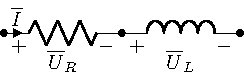
\includegraphics[width=0.83\textwidth]{../figs/RL.pdf}
        \end{center}

        \vspace{-8mm}
        \begin{align*}
            \overline{I} &=I\phase{\theta_I}\\[3pt]
            \overline{U}_R &= R \cdot \overline{I}=R\cdot I\phase{\theta_I}\\[3pt]
        	\overline{U}_L &=\overline{X}_L\cdot\overline{I}= \omega\,L\,I\phase{\theta_I+\ang{90}}
        \end{align*}

        \vspace{-8mm}
        \begin{equation*}
          \quad\; \overline{U} \overarrow[=][\downarrow]{\small 2LK} \overline{U}_R + \overline{U}_L =(\underbrace{R + \mathrm{j}\,\omega L}_{\textstyle \overline{Z}_{eq}} )\; \overline{I} 
          \quad \leftarrow \quad
            \boxed{\text{ \begin{minipage}{0.54\linewidth}\alert{Importante}: sumar\\ módulos en lugar de \\fasores es un \textcolor{red}{error grave} \end{minipage} } }
        \end{equation*}
    \end{column}    
    % Flecha, sacada de aquí: https://tex.stackexchange.com/questions/8720/overbrace-underbrace-but-with-an-arrow-instead
    % "\textstyle" en "underbrace" es para aumentar el tamaño de letra
        
    \begin{column}{0.5\columnwidth}
    \vspace{-22mm}
    
        \hspace{19mm} 
        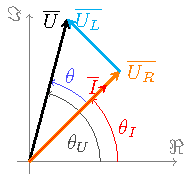
\includegraphics[height=0.57\textheight]{../figs/fasorInductanciaReal_VI.pdf}
        
    \end{column}
    \end{columns}
\end{frame}

%%%%%%%%%%%%%%%

\begin{frame}{Circuito RL \hspace{3mm}(inductivo con pérdidas)}    
    \begin{columns}
    \begin{column}{0.45\columnwidth}
        \vspace{-3mm}
        \begin{center}
            \hspace*{12mm}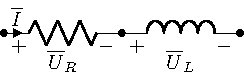
\includegraphics[width=0.83\textwidth]{../figs/RL.pdf}
        \end{center}
        
        \[
            \qquad \overline{Z}_{eq} = R + \mathrm{j}\, \omega L \quad \Rightarrow \quad \boxed{\theta > 0}
        \]

        \[
            \quad\;\; \overline{Z}_{eq} \;
            \begin{dcases}
                |Z_{eq}| = \sqrt{R^2 + (\omega L)^2}\\[5pt]
                \theta = \atan{ \left( \frac{\omega L}{R} \right)}
            \end{dcases}
        \]
        % "dcases" is for not compressing fractions or sqrt, https://tex.stackexchange.com/questions/172693/cases-environment-compresses-fractions        
    \end{column}
    
    \begin{column}{0.55\columnwidth}
        \vspace{15mm}
        \begin{center}
            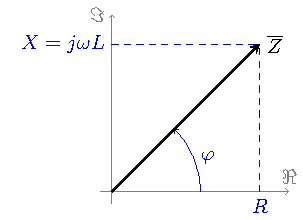
\includegraphics[width=.85\linewidth]{../figs/fasorInductanciaReal.pdf}
        \end{center}
    \end{column}
    \end{columns}
\end{frame}

%%%%%%%%%%%%%%%

\begin{frame}{Circuito RC \hspace{3mm}(capacitivo con pérdidas)}
    %\begin{center}
    %   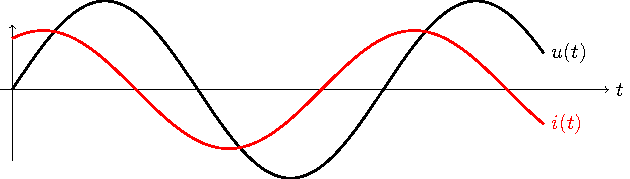
\includegraphics[height=0.25\textheight]{../figs/capacitivo.pdf}
    %\end{center}

    \vspace{3mm}
    \alert{Recordatorio}: por elementos asociados en \alert{serie}, circula la \alert{misma corriente}

    \vspace{1mm}
    \begin{columns}
    \begin{column}{0.5\columnwidth}
    
        \vspace{-3mm}
        \begin{center}
            \hspace*{12mm}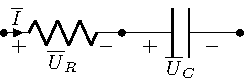
\includegraphics[width=0.81\textwidth]{../figs/RC.pdf}
        \end{center}

        \vspace{-8mm}
        \begin{align*}
            \overline{I} &= I\phase{\theta_I}\\[3pt]
            \overline{U}_R &= R \cdot \overline{I}=R\cdot I\phase{\theta_I}\\[3pt]
        	\overline{U}_C &= \overline{X}_C\cdot\overline{I}= \dfrac{I}{\omega\,C}\phase{\theta_I\ang{-90}}
        \end{align*}
        
        \vspace{-4mm}
        \begin{equation*}
          \quad\; \overline{U} \overarrow[=][\downarrow]{\small 2LK} \overline{U}_R + \overline{U}_C = 
          \Biggl( \overbrace{ R - \mathrm{j}\,\dfrac{1}{\omega C} }^{\textstyle \overline{Z}_{eq}} \Biggl) \; \overline{I}
        \end{equation*}
    \end{column}    
    % Flecha, sacada de aquí: https://tex.stackexchange.com/questions/8720/overbrace-underbrace-but-with-an-arrow-instead
    % "\textstyle" en "underbrace" es para aumentar el tamaño de letra
    
    \vspace{-7mm}
    \begin{column}{0.5\columnwidth}
        \begin{center}
        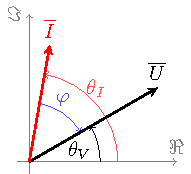
\includegraphics[height=0.6\textheight]{../figs/fasorCondensadorReal_VI.pdf}
        \end{center}
    \end{column}
    \end{columns}
\end{frame}

%%%%%%%%%%%%%%%

\begin{frame}{Circuito RC \hspace{3mm}(capacitivo con pérdidas)}
    \begin{columns}
    \begin{column}{0.45\columnwidth}
        %\vspace{-3mm}
        \begin{center}
            \hspace*{12mm}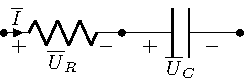
\includegraphics[width=0.83\textwidth]{../figs/RC.pdf}
        \end{center}

        \vspace{-4mm}
        \[
            \qquad \overline{Z}_{eq} =  
            R - \mathrm{j} \frac{1}{\omega C} \quad \Rightarrow \quad \boxed{\theta < 0}
        \]

        \vspace{-4mm}
        \[
            \quad\;\; \overline{Z}_{eq} \;
            \begin{dcases}
                |Z_{eq}| = \sqrt{R^2 + \frac{1}{(\omega C)^2}}\\[5pt]
                \theta = \atan{ \left( \frac{-\,\frac{1}{\omega C} \;}{R} \right)}
            \end{dcases}
        \]
        % "dcases" is for not compressing fractions or sqrt, https://tex.stackexchange.com/questions/172693/cases-environment-compresses-fractions        
    \end{column}
    
    \begin{column}{0.55\columnwidth}
        \vspace{10mm}
        \begin{center}
            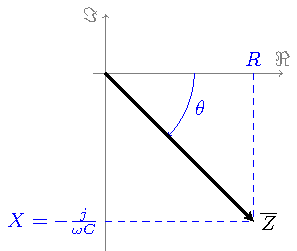
\includegraphics[width=.85\linewidth]{../figs/fasorCondensadorReal.pdf}
        \end{center}
    \end{column}
    \end{columns}
\end{frame}

%%%%%%%%%%%%%%%

\begin{frame}{Circuito RLC serie}
    \vspace{1mm}
    \begin{columns}
    \begin{column}{0.6\columnwidth}
    
        \vspace{1mm}
        \begin{center}
            \hspace*{5mm}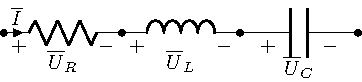
\includegraphics[width=0.9\textwidth]{../figs/RLC.pdf}
        \end{center}

        \vspace{-8mm}
        \begin{align*}
            \overline{I} &=I\phase{\theta_I}\\[3pt]
            \overline{U}_R &= R \cdot \overline{I}=R\cdot I\phase{\theta_I}\\[3pt]
        	\overline{U}_L &=\overline{X}_L\cdot\overline{I}= \omega\,L\,I\phase{\theta_I+\ang{90}}\\[3pt]
            \overline{U}_C &= \overline{X}_C\cdot\overline{I}= \dfrac{I}{\omega\,C}\phase{\theta_I\ang{-90}}
        \end{align*}

        \vspace{-7mm}
        \begin{equation*}
            \;\; \overline{U} \overarrow[=][\downarrow]{\small 2LK}             
            \overline{U}_R + \overline{U}_L + \overline{U}_C = 
            \Biggl( \underbrace{ R + \mathrm{j}\,\omega L - \mathrm{j} \frac{1}{\omega C} }_{\textstyle \overline{Z}_{eq}} \Biggl) \; \overline{I}
        \end{equation*}
    \end{column}    
    % Flecha, sacada de aquí: https://tex.stackexchange.com/questions/8720/overbrace-underbrace-but-with-an-arrow-instead
    % "\textstyle" en "underbrace" es para aumentar el tamaño de letra
        
    \begin{column}{0.4\columnwidth}

    \vspace{8mm}    
        \begin{center}
        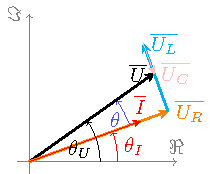
\includegraphics[height=0.55\textheight]{../figs/fasorRLC_VI.pdf}
        \end{center}
        
        \hspace*{7mm}(ejemplo, en el que $X_L > X_C$)
    \end{column}
    \end{columns}
\end{frame}

%%%%%%%%%%%%%%%

\begin{frame}{Circuito RLC serie}
    \begin{columns}
    \begin{column}{0.5\columnwidth}
        %\vspace{-3mm}
        \begin{center}
            \hspace*{3mm}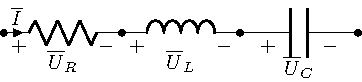
\includegraphics[width=1\textwidth]{../figs/RLC.pdf}
        \end{center}

        \vspace{-4mm}
        \[
            \qquad \overline{Z}_{eq} =  
            R + \mathrm{j} \left( \omega L - \frac{1}{\omega C} \right)            
            \quad \Rightarrow \quad \boxed{ \; \text{?`}\, \theta \,\text{?} \;}
        \]

        \vspace{-4mm}
        \[
            \quad\;\; \overline{Z}_{eq} \;
            \begin{dcases}
                |Z_{eq}| = \sqrt{R^2 + \left( \omega L - \frac{1}{\omega C} \right)^2}\\[5pt]
                \theta = \atan{ \left( \frac{\omega L - \frac{1}{\omega C}}{R} \right)}
            \end{dcases}
        \]
        % "dcases" is for not compressing fractions or sqrt, https://tex.stackexchange.com/questions/172693/cases-environment-compresses-fractions        
    \end{column}
    
    \begin{column}{0.5\columnwidth}
        \vspace{-3mm}
        \hspace*{12mm}(ejemplo, en el que $X_L > X_C$)
        \begin{center}
            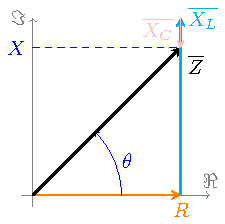
\includegraphics[width=.67\linewidth]{../figs/fasorRLC.pdf}
        \end{center}

        \vspace{-3mm}
        \begin{itemize}
            \item \(\theta > 0 \Rightarrow \omega L > \frac{1}{\omega C}\) : carácter inductivo
            \item \(\theta < 0 \Rightarrow \omega L < \frac{1}{\omega C}\) : carácter capacitivo
            \item \(\theta = 0 \Rightarrow \omega L = \frac{1}{\omega C}\) : carácter resistivo (resonancia)
        \end{itemize}    
    \end{column}
    \end{columns}
\end{frame}

%%%%%%%%%%%%%%%

\begin{frame}{Circuito serie general}
    
    \vspace{4mm}    
    \begin{columns}
    \begin{column}{0.68\linewidth} 
        \hspace{-6mm} 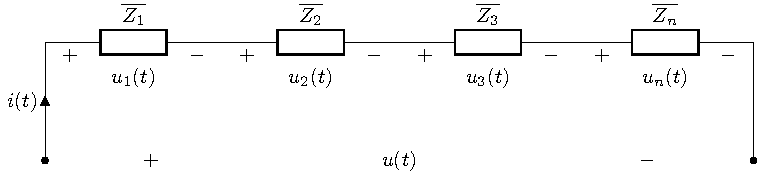
\includegraphics[height=2.5cm]{../figs/serie_general.pdf}
    \end{column}
    \begin{column}{0.03\linewidth}
        \vspace{1mm}

        \hspace*{-3mm}$\LARGE \xrightarrow{\hspace*{0.5cm}}$ % https://latex.org/forum/viewtopic.php?t=3894
    \end{column}
    \begin{column}{0.19\linewidth}
        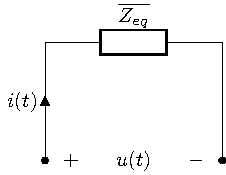
\includegraphics[height=2.5cm]{../figs/serie_general_eq.pdf}
    \end{column}
    \end{columns}

    %\vspace{1mm}
    \begin{equation*}
		\overline{U} \; \underarrow[=][\uparrow]{\vspace{-3mm}\small 2LK} \; \overline{U}_1+\overline{U}_2+...+\overline{U}_n \; = \; \overline{I} \cdot(\overline{Z}_1+\overline{Z}_2+...+\overline{Z}_n) \; = \; \overline{I}\cdot\overline{Z}_{eq}
	\end{equation*}

    \vspace{-6.5mm}
	\begin{equation*}
		\quad\;\; \overline{Z}_{eq}=\overline{Z}_1+\overline{Z}_2+...+\overline{Z}_n\quad \Rightarrow \quad {\Large \boxed{ \overline{Z}_{eq} = \sum_{i=1}^n \overline{Z}_i} }
        \quad \leftarrow \quad
        \boxed{\text{ \begin{minipage}{0.27\linewidth}\alert{Importante}: sumar\\ módulos en lugar de \\fasores es un \textcolor{red}{error grave} \end{minipage} } }
	\end{equation*}

    \vspace{-2mm}
	\begin{equation*}
		R_{eq}=\sum_{i=1}^n R_i\,\qquad \qquad X_{eq}=\sum_{i=1}^n X_i
	\end{equation*}
	\begin{equation*}
		\theta=\arctan\left(\dfrac{X_{eq}}{R_{eq}}\right)
	\end{equation*}
\end{frame}

%%%%%%%%%%%%%%%

\begin{frame}{Ejercicio}
% Circuito serie general
    \vspace{15mm}
    Un circuito serie formado por $R=\qty{10}{\ohm}$, $L=\qty{20}{\milli\henry}$ y $C=\qty{100}{\micro\farad}$ es alimentado con una tensión $u(t)=\qty[parse-numbers = false]{200\cdot\sin\left(1000t+\frac{\pi}{4}\right)}{\volt}$ 

    \vspace{5mm}
    Calcular $\overline{I}$, ${u_R(t)}$, $u_L(t)$ y $u_C(t)$, y dibujar el diagrama fasorial de tensiones y corrientes

    \vspace{17mm}
    \small{\alert{\href{https://raw.githubusercontent.com/ETSIDI-IE/tc/master/docs/ejercicios_clase/TC1_02_Ejemplo_2_5_libro_LBB.pdf}{Solución}}: $\overline{I} = 10\phase{\ang{0}} \,\si{\ampere}$ 

    \hspace{16mm}$u_R(t)=\qty[parse-numbers = false]{100 \sqrt2 \cdot\sin\left(1000t\right)}{\volt}$

    \hspace{16mm}$u_L(t)=\qty[parse-numbers = false]{200 \sqrt2 \cdot\sin\left(1000t+\frac{\pi}{2}\right)}{\volt}$

    \hspace{16mm}$u_C(t)=\qty[parse-numbers = false]{100 \sqrt2 \cdot\sin\left(1000t-\frac{\pi}{2}\right)}{\volt}$}
\end{frame}

%%%%%%%%%%%%%%%

\begin{frame}{Circuito paralelo general}
    \vspace{3mm}
    \alert{Recordatorio}: los elementos asociados en \alert{paralelo} está sometidos a la \alert{misma tensión}

    \vspace{-2mm}
    \begin{columns}
    \begin{column}{0.55\linewidth}
    \begin{center}
        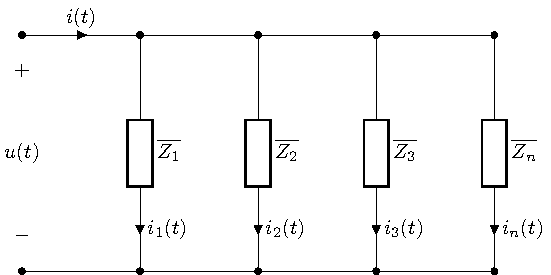
\includegraphics[height=4cm]{../figs/paralelo_general.pdf}
    \end{center}
    \end{column}
    \begin{column}{0.02\linewidth}
        \begin{center}
            $\LARGE \xrightarrow{\hspace*{0.5cm}}$ % https://latex.org/forum/viewtopic.php?t=3894
        \end{center}
    \end{column}
    \begin{column}{0.275\linewidth}
    \begin{center}
        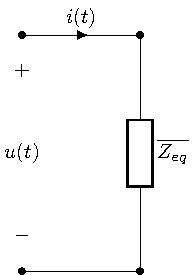
\includegraphics[height=4cm]{../figs/paralelo_general_eq.pdf}
    \end{center}
    \end{column}
    \end{columns}

    \vspace{1mm}
    \begin{equation*}
		\overline{I} \; \underarrow[=][\uparrow]{\vspace{-3mm}\small 1LK} \; \overline{I}_1+\overline{I}_2+...+\overline{I}_n \; = \; \overline{U} \cdot\left(\dfrac{1}{\overline{Z}_1}+\dfrac{1}{\overline{Z}_2}+...+\dfrac{1}{\overline{Z}_n}\right) \; = \; \dfrac{\overline{U}}{\overline{Z}_{eq}}
	\end{equation*}
    \vspace{-4mm}
	\begin{equation*}
		\;\; \dfrac{1}{\overline{Z}_{eq}} = \dfrac{1}{\overline{Z}_1}+\dfrac{1}{\overline{Z}_2}+...+\dfrac{1}{\overline{Z}_n} \quad \Rightarrow \quad \boxed{\dfrac{1}{\overline{Z}_{eq}}=\sum_{i=1}^n \dfrac{1}{\overline{Z}_i}}
	\end{equation*}
\end{frame}

%%%%%%%%%%%%%%%

\begin{frame}{Impedancia y admitancia}
    \begin{columns}
    \begin{column}{0.5\columnwidth}

    \vspace{4mm}
    \begin{center}
        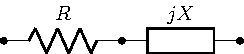
\includegraphics[height=0.12\textheight]{../figs/Z.pdf}
    \end{center}

    \vspace{2mm}
    \begin{align*}
      \overline{U} &= \overline{Z} \cdot \overline{I}\\
      \overline{Z} &= R + j X
    \end{align*}
    \end{column}
    
    \begin{column}{0.5\columnwidth}
    \begin{center}
        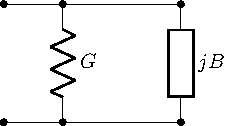
\includegraphics[height=0.25\textheight]{../figs/Y.pdf}
    \end{center}

    \vspace{-5mm}
    \begin{align*}
      \overline{I} &= \overline{Y} \cdot \overline{U}\\
      \overline{Y} &= G + j B
    \end{align*}
    \end{column}
    \end{columns}

    \vspace{5mm}
    \[
    \boxed{\quad 
      \overline{Y} = \frac{1}{\overline{Z}} \quad \rightarrow \quad \left\{%
        \begin{array}{l}
          |\overline{Y}| = \dfrac{1}{|\overline{Z}|}\\[12pt]
          \theta_Y = -\theta_Z \\
          \end{array}\right.
          }
    \]

    \alert{Admitancia}: facilidad que ofrece un circuito al paso de la corriente alterna 
\end{frame}

%%%%%%%%%%%%%%%

\begin{frame}{Impedancia y admitancia}
    \begin{columns}
    \begin{column}{0.5\columnwidth}

    \vspace{4mm}
    \begin{center}
        \includegraphics[height=0.12\textheight]{../figs/Z.pdf}
    \end{center}

    \vspace{7mm}
    \[
      \overline{Z} = \frac{1}{G + \mathrm{j} B} \rightarrow \left\{%
          \begin{array}{l}
        	R = \dfrac{G}{G^2 + B^2}\\[5mm] % Se obtiene al multiplicar numerador y denominador en la expresión de Z por el conjugado del denominador
        	X = \dfrac{-B}{G^2 + B^2}\\
          \end{array}\right.        
    \]
    \end{column}
    
    \begin{column}{0.5\columnwidth}
    \begin{center}
        \includegraphics[height=0.25\textheight]{../figs/Y.pdf}
    \end{center}
    
    \[
      \overline{Y} = \frac{1}{R + \mathrm{j} X} \rightarrow \left\{%
          \begin{array}{l}
        	G = \dfrac{R}{R^2 + X^2}\\[5mm]
        	B = \dfrac{-X}{R^2 + X^2}\\
          \end{array}\right.        
    \]
    \end{column}
    \end{columns}
\end{frame}

%%%%%%%%%%%%%%%%%%%%%%%%%%

\begin{frame}{Ejercicio}
% Impedancia y admitancia
    \vspace{3mm}
    Calcular la impedancia y admitancia compleja equivalente del circuito de la figura
    \begin{figure}[H]
        \centering
        \includegraphics[height=0.64\textheight]{../figs/impedancia_admitancia_eq.pdf}
    \end{figure}

    %\vspace{-2mm}
    \small{\alert{\href{https://raw.githubusercontent.com/ETSIDI-IE/tc/master/docs/ejercicios_clase/TC1_02_Ejemplo_2_7_libro_LBB.pdf}{Solución}}: \hspace{2mm}$\overline{Z} = 18.61\phase{\ang{7.1250}} \,\si{\ohm} \, , \quad \overline{Y} = 0.054\phase{\ang{-7.1250}} \,\si{\per\ohm}$ 
    
    \hspace{17mm}(se recomienda dar hasta 4 decimales en los ángulos)}
\end{frame}

%%%%%%%%%%%%%%%%%%%%%%%%%%

\section{Potencia en corriente alterna}

\begin{frame}{Potencia en CA, \hspace{3mm}expresión general}

    \vspace{1mm}
    Tomemos la tensión como referencia de fases

    \vspace{4mm}
    Sin pérdida de generalidad, asumamos que el ángulo de la impedancia equivalente de un circuito es \(\theta > 0\) (circuito \alert{inductivo}): la corriente está retrasada respecto de la tensión 

    %\vspace{-1mm}
    \begin{align*}
        & \left\{ \begin{array}{l}
            u(t) = U_o \cos (\omega t)\\[8pt]
            i(t) = I_o \cos (\omega t {\color{blue}-} \theta) \quad \text{(circuito en \alert{retraso})} \\
        \end{array} \right.
        \\[14pt]
        & \left. \begin{array}{l}
            \;\;\; p(t) = u(t) \cdot i(t)      
          \end{array} \right.
    \end{align*}
    % To create the brace: https://stackoverflow.com/questions/3412813/multiline-brace-in-eqnarray
\end{frame}

%%%%%%%%%%%%%%%%%%%%%%%%%%

\begin{frame}{Potencia en CA, \hspace{3mm}expresión general}
    \vspace{-15mm} 
    \begin{align*}    
      p(t) &= \underbrace{U_o \cos(\omega t)}_{u(t)} \cdot \underbrace{I_o \cos (\omega t - \theta)}_{i(t)}
      = \underbrace{U_o}_\text{amplitud} \hspace{-3.5mm} \cdot I_o \cdot \cos(\omega t) \cdot \cos(\omega t - \theta) \overarrow[=][\downarrow]{\minibox[c]{\footnotesize conveniente reformular \\[-2pt] \footnotesize \href{https://raw.githubusercontent.com/ETSIDI-IE/tc/master/docs/diapos/TC1_Trigonometria_Complejos_LBB.pdf}{producto de cosenos} }}\\ % para entender este paso, ver pagina 421 del Hayt, 7th edition, English version
      % Flecha, sacada de aquí: https://tex.stackexchange.com/questions/8720/overbrace-underbrace-but-with-an-arrow-instead
      % "Minibox", para poder partir el texto en 2 líneas: https://tex.stackexchange.com/questions/8680/how-can-i-insert-a-newline-in-a-framebox
           &= \frac{1}{2} \cdot U_o \cdot I_o \cdot \left[\cos(2\omega t - \theta) + \cos(\theta)\right]
           = \frac{U_o}{\sqrt{2}} \frac{I_o}{\sqrt{2}} \cdot \left[\cos(2\omega t - \theta) + \cos(\theta)\right]\\
           &= \underbrace{U}_{\substack{\text{valor} \\ \text{eficaz}}} \hspace{-1mm} \cdot I \cdot \left[ \cos(2\omega t - \theta) + \cos(\theta)\right] \underarrow[=][\uparrow]{\footnotesize  \href{https://raw.githubusercontent.com/ETSIDI-IE/tc/master/docs/diapos/TC1_Trigonometria_Complejos_LBB.pdf}{$\cos(\alpha-\beta)$} }\\
           &= U \cdot I \cdot \left[\cos(2\omega t)\cos(\theta) + \sin(2\omega t)\sin(\theta) +  \cos(\theta)\right]
    \end{align*}
    % Para escribir el "underbrace" en varias líneas: https://tex.stackexchange.com/questions/7503/how-can-i-write-multiple-lines-in-a-subscript

    \begin{equation*}
      \boxed{\quad p(t) \;\; = \;\; U \cdot I \cos(\theta) \; + \; U \cdot I \cos(\theta) \cos(2\omega t) \; + \; U \cdot I \sin(\theta) \sin(2\omega t) \quad }
    \end{equation*}
\end{frame}

%%%%%%%%%%%%%%%%%%%%%%%%%%

\begin{frame}{Potencia en CA: \hspace{3mm}potencia activa y potencia reactiva}

    \vspace{2mm}
    En la expresión anterior, definimos dos términos: 
    
    \vspace{1mm}
    \alert{potencia activa} `$P$' y \alert{potencia reactiva} `$Q$'

    \vspace{1mm}
    \begin{equation*}
      p(t) \; = \; {\color{blue}U \cdot I \cos(\theta)} \; + \; {\color{blue}U \cdot I \cos(\theta)} \cos(2\omega t) \; + \; {\color{red}U \cdot I \sin(\theta)} \sin(2\omega t)
    \end{equation*}
    
    \[
      \color{blue}P = U \cdot I\cos\theta \qquad%
      \color{red}Q = U \cdot I\sin\theta
    \]

    \vspace{-5mm}
    
    \begin{equation*}
      \boxed{\quad p(t) \;\; = \;\; {\color{blue}P} \cdot [1 \; + \; \cos(2\omega t)] \; + \; {\color{red}Q} \cdot \sin(2\omega t) \quad}
    \end{equation*}

    \vspace{5mm}

    Pero, ¿qué significa que la potencia sea \textit{activa} o \textit{reactiva}? $\quad \rightarrow \quad$ Siguiente diapositiva
\end{frame}

%%%%%%%%%%%%%%%

\begin{frame}{Potencia en CA: \hspace{3mm}potencia disipada y potencia entretenida} 

    \vspace{2mm}
    Dado que $p(t)$ varía en el tiempo, sus \alert{efectos netos} en el circuito tras cada ciclo pueden calcularse con el \alert{valor medio} en un periodo:
	\begin{equation*}
		P_m \; = \; \dfrac{1}{T}\int_{0}^{T} p(t) \,dt 
        \; = \;
        \dfrac{1}{T} \left[ P \int_{0}^{T} dt \; + \; P \cancelto{0}{\int_{0}^{T} \cos(2\omega t) \,dt} \; + \; Q \cancelto{0}{\int_{0}^{T} \sin(2\omega t) \,dt} \right]
        \; = \;
        \boxed{\, P \,}
	\end{equation*}

    \begin{itemize}
        \item $\boldsymbol{\color{blue!50!black} P} = U\,I\,\cos(\theta)$ es la \alert{potencia neta que se disipa en la carga}, dado que el resto de la potencia $p(t)$ es fluctuante 
        % La potencia fluctuante en las resistencias se debe a que la potencia disipada es mayor cuando circula mayor corriente por las resistencias (en los picos de la senoidal), pero tambien es 0 en algunos instantes (cuando la senoidal cruza por cero en el eje "y")

        \vspace{1mm}
        (Unidades de $P$: \si{\watt})

        \vspace{2mm}
        
        \item $\boldsymbol{\color{blue!50!black} Q} = U\,I\,\sin(\theta)$ es \alert{potencia únicamente \textit{entretenida}}, ya que es potencia almacenada y sucesivamente devuelta por las bobinas y condensadores (para los que $\sin (\theta) \neq 0$)
        %Q es potencia almacenada en las reactancias del circuito (potencia reactiva)

        \vspace{1mm}
        (Unidades de $Q$: \si{\var})
    \end{itemize}    
\end{frame}
	
%%%%%%%%%%%%%%%

\begin{frame}{Potencia en CA, \hspace{3mm}circuito resistivo}
   \[
     P = U\,I \underbrace{\cos\theta}_{=1} \qquad%
     {\color{gray} Q = U\,I}\, \cancelto{0}{{\color{gray} \sin\theta}}
   \]
   
   \begin{equation*}
    p(t) = P \cdot [1 + \cos(2\omega t)] + {\color{gray}Q \cdot \sin(2\omega t)}
    \end{equation*}

    \noindent\rule{\textwidth}{0.5pt}
    \[
      \overline{Z}_R = R \phase{\ang{0}} \;\; \rightarrow \;\; \theta = 0 \;\; \rightarrow \;\; %
      \left\{% 
        \begin{array}{l}
          P = U\,I = \dfrac{U^2}{R} = I^2 R\\
          Q = 0\\
        \end{array}
    \right.
    \]

  \[
    p(t) = P \cdot [1 + \cos(2 \omega t)]
  \]
\end{frame}

%%%%%%%%%%%%%%%

\begin{frame}{Potencia en CA, \hspace{3mm}circuito resistivo}
    \begin{center}
    \includegraphics[width=.9\linewidth]{../figs/resistivoPotencia.pdf}
    \end{center}
    
    \begin{itemize}
    \item Fluctúa al \alert{doble} de \alert{frecuencia} que la tensión y corriente

    \vspace{2mm}
    \item Es siempre \alert{positiva}

    \vspace{2mm}
    \item Su \alert{valor medio} es $P = U\,I\cos\theta = U\,I$ 
    \end{itemize}
\end{frame}

%%%%%%%%%%%%%%%

\begin{frame}{Potencia en CA, \hspace{3mm}circuito inductivo puro}
    \[
        {\color{gray}P = U\,I}\, \cancelto{0}{{\color{gray} \cos\theta}} \qquad%
        Q = U\,I \underbrace{\sin\theta}_{=1} 
    \]
   
    \begin{equation*}
        p(t) = {\color{gray}P \cdot [1 + \cos(2\omega t)]} + Q \cdot \sin(2\omega t)
    \end{equation*}
    
    \noindent\rule{\textwidth}{0.5pt}
    
    \[
        \overline{Z}_L = \omega L \phase{\ang{90}} \;\; \rightarrow \;\; \theta = \frac{\pi}{2} \;\; \rightarrow \;\;%
        \left\{% 
        \begin{array}{l}
          P = 0\\
          Q = U\,I = \dfrac{U^2}{\omega L} = I^2 \omega L\\
        \end{array}
        \right.
    \]

    \[
        p(t) = Q \cdot \sin(2 \omega t)
    \]
\end{frame}

%%%%%%%%%%%%%%%

\begin{frame}{Potencia en CA, \hspace{3mm}circuito inductivo puro}
    \begin{center}
    \includegraphics[width=.86\linewidth]{../figs/inductivoPuroPotencia.pdf}
    \end{center}

    \vspace{-1mm}
    \begin{itemize}
    \item Fluctúa al \alert{doble} de \alert{frecuencia} que la tensión y corriente

    \vspace{2mm}
    \item Pasa por los ceros de tensión y corriente

    \vspace{2mm}
    \item Su valor medio es \alert{nulo}
    \end{itemize}
\end{frame}

%%%%%%%%%%%%%%%

\begin{frame}{Potencia en CA, \hspace{3mm}circuito capacitivo puro}
    \[
        {\color{gray}P = U\,I}\, \cancelto{0}{{\color{gray} \cos\theta}} \qquad%
        Q = U\,I \underbrace{\sin\theta}_{=-1}
    \]
   
    \begin{equation*}
        p(t) = {\color{gray}P \cdot [1 + \cos(2\omega t)]} + Q \cdot \sin(2\omega t)
    \end{equation*}

    \noindent\rule{\textwidth}{0.5pt}

    \[
        \overline{Z}_C = \frac{1}{\omega C} \phase{\ang{-90}} \;\; \rightarrow \;\; \theta = -\frac{\pi}{2} \;\; \rightarrow \;\;%
        \left\{% 
        \begin{array}{l}
            P = 0\\
            Q = -U\,I = -U^2 \omega C = - \dfrac{I^2}{\omega C}\\
        \end{array}
        \right.
    \]
    
    \[
        p(t) = Q \cdot \sin(2 \omega t)
    \]
\end{frame}

%%%%%%%%%%%%%%%

\begin{frame}{Potencia en CA, \hspace{3mm}circuito capacitivo puro}
    \begin{center}
    \includegraphics[width=.86\linewidth]{../figs/capacitivoPuroPotencia.pdf}
    \end{center}
    
    \vspace{-1mm}
    \begin{itemize}
    \item Fluctúa al \alert{doble} de \alert{frecuencia} que la tensión y corriente

    \vspace{2mm}
    \item Pasa por los ceros de tensión y corriente

    \vspace{2mm}
    \item Su valor medio es \alert{nulo}
    \end{itemize}
\end{frame}

%%%%%%%%%%%%%%%

\begin{frame}{Potencia en CA, \hspace{3mm}circuito inductivo con pérdidas (RL)}
    \vspace{5mm}
    \begin{center}
        \includegraphics[height=0.7\textheight]{../figs/inductivoPotencia.pdf}
    \end{center}
    
    %\[
    %     p(t) = P \cdot [1 + \cos(2\omega t)] + Q \cdot \sin(2\omega t)
    %\]
    
    %\begin{center}
    %    Valor medio positivo, \(P = U I \cos \theta\)
    %\end{center}
\end{frame}

%%%%%%%%%%%%%%%

\begin{frame}{Potencia en CA, \hspace{3mm}circuito capacitivo con pérdidas (RC)}
    \vspace{5mm}
    \begin{center}
        \includegraphics[height=0.68\textheight]{../figs/capacitivoPotencia.pdf}
    \end{center}
    
    %\[
    %     p(t) = P \cdot (1 + \cos(2\omega t)) + Q \cdot \sin(2\omega t)
    %\]
    
    %\begin{center}
    %    Valor medio positivo, \(P = U I \cos \theta\)
    %\end{center}
\end{frame}

%%%%%%%%%%%%%%%

\begin{frame}{Interludio: \hspace{8mm}pasado y presente de los sistemas eléctricos}    
    \begin{minipage}[c]{0.25\linewidth}
        \begin{center}            
            \vspace{3mm}
            \href{https://www.youtube.com/watch?v=aefuvLBxQyM}{Ms. Edith Clarke}, 
            
            General Electric

            \vspace{3mm}
            \includegraphics[width=1\linewidth]{../figs/edith_clarke.jpg}
        \end{center}
    \end{minipage}
    \hfill%
    \begin{minipage}[c]{0.3\linewidth}
        \begin{center}    
            \vspace{-4mm}
            \href{https://www.youtube.com/watch?v=Sr4qD9G8jeY}{Prof. Gabriela Hug}, 
            
            ETH Zurich

            \vspace{3mm}
            \includegraphics[width=1\linewidth]{../figs/gabriela_hug.png}
        \end{center}
    \end{minipage}    
    \hfill%
    \begin{minipage}[c]{0.3\linewidth}
        \begin{center}    
            \vspace{-8.5mm}
            \href{https://www.youtube.com/watch?v=YlLlAyELKng}{Dr Vera Silva}, 
            
            General Electric

            \vspace{3mm}
            \includegraphics[width=1\linewidth]{../figs/vera_silva.jpg}
        \end{center}
    \end{minipage}
\end{frame}

%%%%%%%%%%%%%%%

\begin{frame}{Triángulo de potencias}
    \begin{columns} 
    \begin{column}{0.6\columnwidth}
    \vspace{2mm}
    \begin{itemize}
        \item Potencia \alert{activa} [W]
    \end{itemize}
    \[  
        \boxed{P = U\cdot I\cdot\cos(\theta) = R \cdot I^2}
    \]
    
    \begin{itemize}
        \item Potencia \alert{reactiva} [VAr]
    \end{itemize}
    \[
        \boxed{Q = U\cdot I\cdot\sin(\theta) = X \cdot I^2}
    \]
    
    \begin{itemize}
        \item Potencia \alert{aparente} [VA]
    \end{itemize}
    \[
        \boxed{\overline{S} = P + \mathrm{j}Q = \overline{U} \cdot \overline{I}^*}
    \]
    
    \hspace{8mm}Demostración de la expresión para $\overline{S}$:

    \vspace{-7mm}
    {\begin{align*}
        \overline{U} &= U\phase{0}\\
        \overline{I} &= I\phase{-\theta} \quad \text{(circuito en retraso)}\\
        \overline{U}\cdot\overline{I}^* &= U\phase{0} \cdot I\phase{\theta} = U\,I\phase{\theta}=\\
        &=U\,I\, (\cos\theta + \mathrm{j} \sin\theta) = P + \mathrm{j} Q
    \end{align*}}
    \end{column}
    
    \begin{column}{0.4\columnwidth}
    \vspace{-3mm}
    
        \hspace{-15mm}
        \includegraphics[width=1.2\linewidth]{../figs/trianguloPotencias.pdf}    
    
    \[
        S = U \cdot I
    \]
    \[
        \theta_S = \theta_Z = \theta
    \]
    
    %\vspace{2mm}
    
    %Definimos el \textit{factor de potencia}:
    %\vspace{-3mm}
    
    %\[
    %    \text{f.d.p.} \equiv \cos(\theta)
    %\]
    \end{column}
    \end{columns}
\end{frame}

%%%%%%%%%%%%%%%

\begin{frame}{Triángulo de potencias}
    \begin{columns} 
    \begin{column}{0.6\columnwidth}
    \vspace{2mm}
    \begin{itemize}
        \item Potencia \alert{activa} [W]
    \end{itemize}
    \[  
        \boxed{P = U\cdot I\cdot\cos(\theta) = R \cdot I^2}
    \]
    
    \begin{itemize}
        \item Potencia \alert{reactiva} [VAr]
    \end{itemize}
    \[
        \boxed{Q = U\cdot I\cdot\sin(\theta) = X \cdot I^2}
    \]
    
    \begin{itemize}
        \item Potencia \alert{aparente} [VA]
    \end{itemize}
    \[
        \boxed{\overline{S} = P + \mathrm{j}Q = \overline{U} \cdot \overline{I}^*}
    \]
    
    \hspace{8mm}Demostración de la expresión para $\overline{S}$:

    \vspace{-7mm}
    {\begin{align*}
        \overline{U} &= U\phase{0}\\
        \overline{I} &= I\phase{-\theta} \quad \text{(circuito en retraso)}\\
        \overline{U}\cdot\overline{I}^* &= U\phase{0} \cdot I\phase{\theta} = U\,I\phase{\theta}=\\
        &=U\,I\, (\cos\theta + \mathrm{j} \sin\theta) = P + \mathrm{j} Q
    \end{align*}}
    \end{column}
    
    \begin{column}{0.4\columnwidth}
    \vspace{-3mm}
    
        \hspace{-15mm}
        \includegraphics[width=1.2\linewidth]{../figs/reactive_power_beer.png}    
    
    \end{column}
    \end{columns}
\end{frame}

%%%%%%%%%%%%%%%

\begin{frame}{Potencia en elementos: \hspace{3mm}resistencia}
    \[
    \theta = 0 \quad \Rightarrow \quad
    \begin{cases}
      P_R = R \, I^2\\[4pt]
      Q_R = 0\\[4pt]
      S_R = P_R
    \end{cases}
    \]
    
    \begin{itemize}
        \item Consume potencia activa

        \vspace{2mm}
        \item No ``consume'' potencia reactiva
    \end{itemize}
\end{frame}

%%%%%%%%%%%%%%%

\begin{frame}{Potencia en elementos: \hspace{3mm}inductancia}
    \[
    \theta = \pi/2 \quad \Rightarrow \quad
    \begin{cases}
      P_L = 0\\[4pt]
      Q_L = \omega L\, I^2\\[4pt]
      \overline{S}_L = \omega L\, I^2 \phase{\pi/2}
    \end{cases}
    \]
    
    \begin{itemize}
        \item No consume potencia activa

        \vspace{2mm}
        \item ``Consume'' potencia reactiva (\(Q > 0\))
        
        \vspace{2mm}
        \begin{itemize}
            \item {\normalsize \alert{Nota}: la potencia reactiva es potencia \textit{entretenida}, no es potencia que se consuma}

            \vspace{2mm}
            {\normalsize Pero, dado el convenio de signos, decimos que \alert{las bobinas ``consumen'' $Q$} y \alert{los condensadores ``generan'' $Q$} (ya que almacenan y devuelven energía al circuito en semiciclos opuestos)}
        \end{itemize}
    \end{itemize}
\end{frame}

%%%%%%%%%%%%%%%

\begin{frame}{Potencia en elementos: \hspace{3mm}condensador}
    \[
    \theta = - \pi/2 \quad \Rightarrow \quad 
    \begin{cases}
      P_L = 0\\[4pt]
      Q_C = - \omega C\, U^2\\[4pt]
      \overline{S}_C = \omega C \, U^2 \phase{-\pi/2}
    \end{cases}
    \]
    
    \begin{itemize}
        \item No consume potencia activa
        
        \vspace{2mm}
        \item ``Genera'' potencia reactiva (\(Q < 0\))

        \vspace{2mm}
        \begin{itemize}
            \item {\normalsize \alert{Nota}: la potencia reactiva es potencia \textit{entretenida}, no es potencia que se consuma}

            \vspace{2mm}
            {\normalsize Pero, dado el convenio de signos, decimos que \alert{las bobinas ``consumen'' $Q$} y \alert{los condensadores ``generan'' $Q$} (ya que almacenan y devuelven energía al circuito en semiciclos opuestos)}
        \end{itemize}
        % Se dice que los condensadores "entregan" o "generan" potencia reactiva. En realidad, esto es un convenio, porque las cargas suelen ser inductivas y por eso se compensa el factor de potencia con condensadores. Pero si las cargas por el contrario fueran capacitivas, probablemente diríamos que son las bobinas las que "entregan" potencia reactiva, porque serían las que usaríamos para compensar el factor de potencia. Está bien explicado aquí: https://www.quora.com/Why-does-an-inductor-consume-reactive-power-while-a-capacitor-generates-reactive-power
    \end{itemize}
\end{frame}

%%%%%%%%%%%%%%%

\begin{frame}{Teorema de Boucherot}
    \vspace{3mm}
    En un circuito con múltiples elementos, la potencia aparente total es la \alert{suma de las potencias aparentes individuales} 
    
    (la potencia activa/reactiva total es la \alert{suma de las potencias activas/reactivas individuales})
    
    \begin{columns}
    \begin{column}{0.3\columnwidth}
    
        \vspace{-11mm}
        
        \begin{align*}          
          P_T + \mathrm{j}Q_T &= \sum^n_{i = 1} (P_i + \mathrm{j}Q_i)\\
          \overline{S}_T &= \sum_{i = 1}^{n} \overline{S}_i
        \end{align*}

        \vspace{-3mm}
        
        \begin{align*}
            P_T &= \sum_{i = 1}^n P_i\\
            Q_T &= \sum_{i = 1}^n Q_i
        \end{align*}
    \end{column}
    \begin{column}{0.7\linewidth}
        \begin{figure}
        \vspace{-10mm}
    
        \hspace*{-18mm}  \includegraphics[width=1.18\linewidth]{../figs/boucherot.pdf}
        \end{figure}
    \end{column}
    \end{columns}
\end{frame}

%%%%%%%%%%%%%%%

%\begin{frame}{Teorema de Boucherot}
%    \vspace{2mm}
%    \begin{itemize}
%        \item Consecuencia del \alert{principio de conservación de la energía}
%    
%        \vspace{2mm}
%        
%        \item Supóngase $\overline{Z_1}=R_1+\mathrm{j}\,X_1$, $\overline{Z_2}=R_2+\mathrm{j}\,X_2$ y $\overline{Z_3}=R_3-\mathrm{j}\,X_3$ en serie recorridas por $\overline{I}=I\phase{0^\circ}$:
%        \begin{equation*}
%            \overline{U} \overarrow[=][\downarrow]{\vspace{-1mm}\small 2LK} \sum_{i=1}^3 \overline{U_i}\Rightarrow
%            \begin{cases}
%                U\,\cos(\theta)=\displaystyle\sum_{i=1}^3 U_i\,\cos(\theta_i)\\
%                U\,\sin(\theta)=\displaystyle\sum_{i=1}^3 U_i\,\sin(\theta_i)
%            \end{cases}
%        \end{equation*}
%        Multiplicando ambas expresiones por ${I}$: 
%        \begin{align*}
%            U\,I\,\cos(\theta)&=P_T=\displaystyle\sum_{i=1}^3 U_i\,I\,\cos(\theta_i)=\displaystyle\sum_{i=1}^3 P_i\\
%            U\,I\,\sin(\theta)&=Q_T=\displaystyle\sum_{i=1}^3 U_i\,I\,\sin(\theta_i)=\displaystyle\sum_{i=1}^3 Q_i
%        \end{align*}
%    \end{itemize}
%\end{frame}

%%%%%%%%%%%%%%%

\begin{frame}{Ejercicio}
% Teorema de Boucherot

    \vspace{5mm}
    Sabiendo que las fuentes de tensión del circuito de la figura vienen definidas por las formas de onda $u_1(t)=10\sqrt{2}\cdot \cos(1000\cdot t) \,\si{\volt}$ y $u_2(t)=5\sqrt{2}\cdot \sin(1000\cdot t) \,\si{\volt}$, se debe calcular las potencias de cada elemento, así como el balance de potencias del circuito 
		\begin{figure}[H]
			\centering
			\includegraphics[width=0.6\linewidth]{../figs/ej7_BT2.pdf}
		\end{figure}

  \alert{Solución}: \href{https://raw.githubusercontent.com/ETSIDI-IE/tc/master/docs/ejercicios_clase/TC1_02_Ejemplo_2_9_libro_LBB.pdf}{aquí}
\end{frame}

%%%%%%%%%%%%%%%

\begin{frame}{Medida de potencia: \hspace{3mm}vatímetro}
    \vspace{3mm}
    \begin{center}
        \includegraphics[height=0.5\textheight]{../figs/vatimetro_2.pdf}
    \end{center}

    \vspace{2mm}
    
    \centering Equipo de medida de \alert{4 terminales} (un par para tensión, un par para corriente)

    \vspace{-4mm}
    \begin{equation*}
        W \; = \; \hspace{-2mm} \underbrace{ \overline{I}_{1,2}\,\bullet\,\overline{U}_{3,4} }_{\substack{\text{producto escalar}}} \hspace{-2mm} \; = \;  
        I_{1,2}\cdot U_{3,4}\cdot \cos\widehat{(\overline{I}_{1,2}, \overline{U}_{3,4})}
	\end{equation*}
\end{frame}

%%%%%%%%%%%%%%%

\begin{frame}{Medida de potencia}
    \begin{center}
        \includegraphics[height=0.5\textheight]{../figs/vatimetro_Z.pdf}
    \end{center}

    \vspace{2mm}
    
    \centering Habitualmente se emplea con 3 terminales, \alert{cortocircuitando} terminales con *

    \vspace{-3mm}
    \[
      \boxed{\; W \; = \; |\overline{V}| \cdot |\overline{I}| \cdot \cos(\theta_V - \theta_I) \; = \; P_Z \;}
    \]
\end{frame}

%%%%%%%%%%%%%%%

\subsection{Factor de potencia: importancia y mejora}

\begin{frame}{Factor de potencia}
    El factor de potencia (\textit{\alert{f.d.p.}}), \(\cos(\theta)\), representa la aportación de potencia activa dentro de la potencia aparente:
    \[
        \cos (\theta)=\dfrac{P}{S}
    \]

    Se dice que:
	\begin{itemize}
		\item \textit{fdp} \alert{en retraso} cuando el circuito tiene carácter inductivo (la intensidad va retrasada respecto a la tensión)

        \vspace{2mm}
		\item \textit{fdp} \alert{en adelanto} cuando el circuito tiene carácter capacitivo (la intensidad va adelantada respecto a la tensión)
	\end{itemize}	
\end{frame}

%%%%%%%%%%%%%%%

\begin{frame}{Factor de potencia: \hspace{3mm}importancia y mejora}
    Sean dos sistemas con \alert{misma tensión y potencia activa}, y factores de potencia \(\cos \theta_2 < \cos \theta_1 \;\) (\(Q_2 > Q_1\))
    \begin{columns}
    \begin{column}{0.4\linewidth}    
        \hspace{-3mm}\includegraphics[width=1.05\linewidth]{../figs/fasorescompensacionreactiva.pdf}
    \end{column}
    \begin{column}{0.6\linewidth}
    \begin{itemize}
        \item El sistema 2 requiere \alert{mayor potencia aparente} (generador mayor) para alimentar la misma potencia activa:
        \[
          \left(\frac{P}{\cos \theta_1} = S_1 \right) < \left( S_2 = \frac{P}{\cos \theta_2}\right) 
        \]
        \item El sistema 2 requiere \alert{mayor sección de cable} para transportar la misma potencia activa:
        \[
          \left(\frac{P}{U \cos \theta_1} = I_1 \right) < \left( I_2 = \frac{P}{U \cos \theta_2}\right) 
        \]
    \end{itemize}
    \end{column}
    \end{columns}
\end{frame}

%%%%%%%%%%%%%%%

\begin{frame}{``Generación'' local de reactiva}
    \begin{itemize}
    \item Comúnmente, el factor de potencia es \alert{inductivo} (máquinas eléctricas
    industriales)

    \vspace{5mm}
    \item La red debe suministrar potencia reactiva inductiva (influye en secciones de líneas y tamaños de generadores $\rightarrow$ \alert{mayor coste})

    \vspace{5mm}
    \item Es necesario mejorar \alert{localmente} el factor de potencia

    \vspace{2mm}
    Solución
    común: utilizar \alert{bancos de condensadores} como suministradores de
    $Q$
    \end{itemize}
\end{frame}

%%%%%%%%%%%%%%%

\begin{frame}{Cálculo de la capacidad para compensación de reactiva}
    \vspace{2mm}
    Sea una carga de potencia activa \(P_z\), potencia reactiva \(Q_z\), factor de potencia \(\cos\theta\) 

    \vspace{-1mm}
    Se desea \alert{mejorar el factor de potencia} a \(\cos \theta' > \cos \theta\), 
    \href{https://raw.githubusercontent.com/ETSIDI-IE/tc/master/docs/ejercicios_clase/TC1_02_conexion_paralelo_reactiva.pdf}{manteniendo la potencia \(P_z\)} 

    \vspace{-4mm}
    \begin{columns}
    \begin{column}{0.4\linewidth}
        \begin{center}
            \includegraphics[width=0.9\linewidth]{../figs/circuitocompensacionreactiva.pdf}
        \end{center}

        \vspace{-5mm}
        \begin{center}
            \includegraphics[width=0.6\linewidth]{../figs/trianguloCompensacionQ.pdf}
        \end{center}
    \end{column}
    \begin{column}{0.6\linewidth}

        \vspace{-1mm}
        \begin{align*}
          P' &= P_z\\
          Q' &= Q_c + Q_z \quad (Q' < Q_z)\\
          \overline{I}' &= \overline{I}_c + \overline{I}_z \quad (I' < I_z)\\
        \end{align*}

        \vspace{-10mm}
        \begin{align*}
            Q_z &= P_z \tan \theta\\
            Q'&= P_z \tan \theta'\\
            |Q_c| &= Q_z - Q' = P_z (\tan \theta - \tan \theta')
        \end{align*}

        \vspace{-9mm}
        \[
            |Q_c| = \underbrace{X_c \,\cdot}_{=\frac{1}{\omega C}} I_c^2 = \omega C U^2 \rightarrow \boxed{C = \frac{P_z (\tan \theta - \tan \theta')}{\omega U^2}}
        \]
    \end{column}
    \end{columns}
\end{frame}

%%%%%%%%%%%%%%%

\section{Teoremas}

\begin{frame}{Equivalencia de fuentes}

    \vspace{3mm}
    Sólo es posible establecer \alert{equivalencia} entre \alert{fuentes reales}

    (la deducción es equivalente a la ya vista para corriente continua)

    \vspace{-2mm}
    \begin{columns}
    \begin{column}{0.33\columnwidth}
    \begin{center}
        \includegraphics[height=0.5\textheight]{../figs/FuenteTensionReal.pdf}
    \end{center}
    \[
      \overline{U}_{AB} = \overline{\epsilon}_g - \overline{Z}_{\epsilon_g} \cdot \overline{I}
    \]
    \end{column}
    \begin{column}{0.33\columnwidth}
    \begin{align*}
      \overline{Z}_g &= \overline{Z}_{\epsilon_g} = \overline{Z}_{I_g}\\[3mm]
      \overline{\epsilon}_g &= \overline{Z}_g \cdot \overline{I}_g\\[3mm]
      \overline{I}_g &= \frac{\overline{\epsilon}_g}{\overline{Z}_g}
    \end{align*}
    \end{column}
    \begin{column}{0.33\columnwidth}
    \begin{center}
        \includegraphics[height=0.5\textheight]{../figs/FuenteCorrienteReal.pdf}
    \end{center}
    \[
      \overline{I} = \overline{I}_g - \frac{\overline{U}_{AB}}{\overline{Z}_{I_g}}
    \]
    \end{column}
    \end{columns}
\end{frame}

%%%%%%%%%%%%%%%

\subsection{Principio de superposición}

\begin{frame}{Superposición}

    \vspace{3mm}
    La respuesta de un \alert{circuito lineal} a varias fuentes de excitación actuando simultáneamente es igual a la \alert{suma de las respuestas} que se tendrían cuando actuase cada una de ellas por separado

    \vspace{-2mm}
    \[
        y(t) = \sum_i y_i(t)
    \]

    %\vspace{-2mm}
    \begin{minipage}[c]{0.45\linewidth}
        \begin{center}
            \includegraphics[width=0.88\linewidth]{../figs/superposicion2.pdf}
        \end{center}
    \end{minipage}
    \hfill%
    \begin{minipage}[c]{0.45\linewidth}
        \begin{center}
            \includegraphics[width=0.95\linewidth]{../figs/superposicion.pdf}
        \end{center}
    \end{minipage}
\end{frame}

%%%%%%%%%%%%%%%

\begin{frame}{Análisis de un circuito mediante superposición}
    \begin{block}{Procedimiento}
    \vspace{1mm}
    
    \begin{enumerate}
        \item Se \alert{eliminan} todas las \alert{fuentes independientes} del circuito menos una
        \vspace{1mm}
        
        \begin{itemize}
            \normalsize{
            \item Las fuentes de \alert{tensión} se sustituyen por un \alert{cortocircuito} (\(U = 0\))
            \vspace{1mm}
            
            \item Las fuentes de \alert{corriente} se sustituyen por un \alert{circuito abierto} (\(I = 0\))
            \vspace{1mm}
            
            \item Las fuentes \alert{dependientes no se modifican}
            }
        \end{itemize}
        \vspace{2mm}
        
        \item Se analiza el circuito, obteniendo la \alert{respuesta individual} a la fuente que permanece activa
        \vspace{2mm}
        
        \item Se repite este procedimiento para \alert{cada una de las fuentes independientes} del circuito
        \vspace{2mm}
        
        \item La respuesta total del circuito es la \alert{suma de las respuestas individuales}
    \end{enumerate}
    \vspace{1mm}
    \end{block}
\end{frame}

%%%%%%%%%%%%%%%

\begin{frame}{Análisis de un circuito mediante superposición}

    \begin{block}{Observaciones}
    \begin{itemize}
        \vspace{2mm}
        \item \alert{Siempre} hay que \alert{aplicar este método} cuando en un circuito conviven \alert{fuentes de distinta frecuencia} (o fuentes de corriente continua y corriente alterna)

        \vspace{2mm}
        \item En el caso de fuentes de \alert{corriente alterna senoidal}:

        \vspace{1mm}
        \begin{itemize}
            \normalsize{\item \alert{Para cada frecuencia}, las bobinas y condensadores presentarán \alert{diferente reactancia}, por lo que habrá que calcularlas
            
            \vspace{1mm}
            \item La respuesta total debe expresarse en el \underline{\alert{dominio del tiempo}}
            
            \vspace{1mm}
            (\alert{\textcolor{red}{NO}} se pueden \alert{sumar fasores} que corresponden a \alert{frecuencias diferentes})
            }
        \end{itemize}
        
        \vspace{2mm}
        \item En el primer paso del procedimiento, se pueden \alert{agrupar las fuentes que funcionan a la misma frecuencia} y calcular la respuesta del circuito en esa frecuencia

        \vspace{1mm}
    \end{itemize}
    \end{block}
\end{frame}

%%%%%%%%%%%%%%%

\begin{frame}{Recordatorio: \hspace{3mm}el cálculo fasorial es válido para señales de igual $\omega$} \label{diapo:fasores_distintaFrecuencia}

    \begin{center}
        \includegraphics[height=0.6\textheight]{../figs/Fasor_distintasFrecuencias_1.pdf}
    \end{center}
\end{frame}

%%%%%%%%%%%%%%%

\begin{frame}{...pero \textcolor{red}{NO} para señales de distinta frecuencia ($\omega_1 \neq \omega_2$)}

    \begin{center}
        \includegraphics[height=0.6\textheight]{../figs/Fasor_distintasFrecuencias_2.pdf}
    \end{center}
\end{frame}

%%%%%%%%%%%%%%%

\begin{frame}{Principio de superposición y potencia}
    El principio de superposición aplica a tensiones y corrientes, pero \alert{NO a potencias}
    
    (ya que potencia es el resultado de una \alert{operación no lineal}, el producto de corriente y tensión)

    \vspace{5mm}
    
    Supongamos \(i(t) = i_1(t) + i_2(t)\):
    \begin{align*}
      p(t) &= R \cdot i^2(t) =\\[2pt]
           &= R \cdot [i_1(t) + i_2(t)]^2 =\\[4pt]
           &=R \cdot [i_1^2(t) + i_2^2(t) + 2\cdot i_1(t) \cdot i_2(t)]\\[4pt] % El último sumando es 0 para señales ortogonales (ver la definición de señales ortogonales en la siguiente diapositiva)
     \Aboxed{\; p(t) \; &\textcolor{red}{\neq} \; p_1(t) + p_2(t) \;}
    \end{align*}
\end{frame}

%%%%%%%%%%%%%%%

\begin{frame}{Principio de superposición y potencia}
    \begin{itemize}
        \item Cuando las señales son \alert{ortogonales en un periodo}\footnote{Dos señales son ortogonales si cumplen la siguiente propiedad: \[<f_1, f_2>_T \;\; = \int_T \; f_1(t) \cdot f_2(t) \; dt = 0\]} se pueden sumar las \alert{potencias medias} de cada circuito:
        % Si f1 y f2 son senoidales de distinta fecuencia, hay que calcular la integral en el periodo "T", siendo este "T" el periodo de la señal con mayor periodo de las dos
    \end{itemize}
    \begin{align*}
      P = \sum_i P_i
    \end{align*}
    \begin{itemize}
        \item Ejemplos de señales ortogonales: 
        
        senoidales con diferente frecuencia, una senoidal con una continua\ldots{}
    \end{itemize}
\end{frame}

%%%%%%%%%%%%%%%

\begin{frame}{Principio de superposición y potencia}

    \vspace{1mm}
    \begin{itemize}
        \item Cuando las señales son \alert{ortogonales en un periodo}, se pueden sumar las \alert{potencias medias} de cada circuito:
        % Si f1 y f2 son senoidales de distinta fecuencia, hay que calcular la integral en el periodo "T", siendo este "T" el periodo de la señal con mayor periodo de las dos
    \end{itemize}
    \begin{align*}
      P_m \;\; &= \;\; \dfrac{1}{T} \int_{T} p(t) \,dt 
        \;\; = %\;\; \dfrac{1}{T} \int_{T} R \cdot i^2(t) \;dt \;\; = \;\; R \cdot \dfrac{1}{T} \int_{T} \; [i_1(t) + i_2(t)]^2 \;dt \;\; =
        \\[2pt]
           &= \;\; R \cdot \dfrac{1}{T} \bigg[ 
           \int_{T} i_1^2(t) \;dt \;+\; 
           \int_{T} i_2^2(t) \;dt \;+\;
           \underbrace{\cancelto{0}{\int_{T} 2\cdot i_1(t) \cdot i_2(t) \;dt \;\;}}_{\text{señales ortogonales}}
           \hspace*{-2.5mm}\bigg] \;\; = \\
           &= \;\; R \cdot \big( \underbrace{I_1^2 + I_2^2}_{\substack{\text{valores} \\ \text{\hyperlink{diapo:valorEficaz_definicion}{eficaces}}}} \big) \;\; = \;\; \boxed{P_1 + P_2}
    \end{align*}
    % Para escribir el "underbrace" en varias líneas: https://tex.stackexchange.com/questions/7503/how-can-i-write-multiple-lines-in-a-subscript
\end{frame} 

%%%%%%%%%%%%%%%

\begin{frame}{Principio de superposición y potencia: \hspace{3mm}ejemplo}

    \vspace{3mm}
    Teniendo en cuenta la propiedad de ortogonalidad, si en un circuito actúan \alert{fuentes de continua} y \alert{varias fuentes de alterna} de \alert{distinta frecuencia} entre ellas:

    \vspace{2mm}
    \begin{itemize}
        \item Potencia disipada en una \alert{resistencia}:

        \vspace{-4mm}
        \begin{equation*}
            {P_R=R\cdot\left(I_{cc}^2+I_1^2+I_2^2+...+I_n^2 \right)}
        \end{equation*}

        \vspace{2mm}
        \item \alert{Potencia entregada por fuente de tensión} de frecuencia $\omega_1$: 
        \begin{equation*}
            {P=E\,I_1\,\cos(\theta_{i_1})}
        \end{equation*}

        \vspace{2mm}
        \item \alert{Potencia entregada por fuente de corriente} de frecuencia $\omega_2$: 
        \begin{equation*}
            {P=U_2\,I_{g}\,\cos(\theta_{u_2})}
        \end{equation*}
        
        \vspace*{2mm}
        \fbox{ \begin{minipage}{0.9\linewidth} 
        \hspace{3mm}
        \alert{Potencia entregada}: 

        \hspace{3mm}
        solo actúa la componente de la intensidad/tensión que tiene \alert{la misma} 

        \hspace{3mm}
        \alert{frecuencia} que el generador de tensión/corriente
        \end{minipage} }
    \end{itemize}
\end{frame}

%%%%%%%%%%%%%%%

\subsection{Teoremas de Thévenin y Norton}

\begin{frame}{Teorema de Thévenin}
    \vspace{3mm}
    Cualquier \alert{red lineal} compuesta por elementos activos y pasivos puede sustituirse, desde el punto de vista de sus terminales externos A-B, por una \alert{fuente de tensión} (generador de Thévenin, \(\epsilon_{th}\)) en \alert{serie} con una impedancia (impedancia de Thévenin, \(Z_{th}\))
    % Importante: los equivalentes de Thévenin y Norton, y los resultados del teorema de la máxima transferencia de potencia, solo son válidos para la frecuencia a la que han sido calculados.

    \vspace{2mm}
    \begin{center}
        \includegraphics[height=0.6\textheight]{../figs/EquivalenteThevenin.pdf}
    \end{center}
\end{frame}

%%%%%%%%%%%%%%%

\begin{frame}{Cálculo del equivalente de Thévenin}
    \vspace{2mm}
    \begin{center}
        \includegraphics[height=0.43\textheight]{../figs/EquivalenteThevenin0.pdf}
    \end{center}
    
    \begin{itemize}
        \item Circuito abierto (\(Z_L \to \infty, \quad U_{AB} = U_{oc}\))
    \end{itemize}
    
    \vspace{-5mm}
    \[
        \hspace{65mm}
        \boxed{\epsilon_{th} = U_{oc}} 
        \qquad \textrm{(\small{SC$\equiv$\textit{short circuit}, \hspace*{4mm}OC$\equiv$\textit{open circuit}})}
    \] 
    
    \vspace{-1mm}
    \begin{itemize}
        \item Cortocircuito (\(Z_L = 0, \quad I = I_{sc}\))
    \end{itemize}
    \[
        \boxed{Z_{th} = \frac{\epsilon_{th}}{I_{sc}} = \frac{U_{oc}}{I_{sc}}}
    \]
\end{frame}

%%%%%%%%%%%%%%%

\begin{frame}{Teorema de Norton}
    \vspace{3mm}
    Cualquier \alert{red lineal} compuesta por elementos activos y pasivos puede sustituirse, desde el punto de vista de sus terminales externos A-B, por una \alert{fuente de corriente} (generador de Norton, \(I_N\)) en \alert{paralelo} con una impedancia (impedancia de Norton, \(Z_N\))
    % Importante: los equivalentes de Thévenin y Norton, y los resultados del teorema de la máxima transferencia de potencia, solo son válidos para la frecuencia a la que han sido calculados.

    \vspace{2mm}
    \begin{center}
        \includegraphics[height=0.6\textheight]{../figs/EquivalenteNorton.pdf}
    \end{center}
\end{frame}

%%%%%%%%%%%%%%%

\begin{frame}{Cálculo del equivalente de Norton}

    \vspace{2mm} 
    \begin{center}
        \includegraphics[height=0.43\textheight]{../figs/EquivalenteNorton.pdf}
    \end{center}
    
    \begin{itemize}
        \item Cortocircuito (\(Z_L = 0, \quad I = I_{sc}\))
    \end{itemize}

    \vspace{-8mm}
    \[
        \hspace{65mm}
        \boxed{I_N = I_{sc}}
        \qquad \textrm{(\small{SC$\equiv$\textit{short circuit}, \hspace*{4mm}OC$\equiv$\textit{open circuit}})}
    \]  
    
    \vspace{1mm}
    \begin{itemize}
        \item Circuito abierto (\(Z_L \to \infty, \quad U_{AB} = U_{oc}\))
    \end{itemize}
    \[
        \boxed{Z_N = \frac{U_{oc}}{I_N} = \frac{U_{oc}}{I_{sc}}}
    \]
\end{frame}

%%%%%%%%%%%%%%%

\begin{frame}{Cálculo de impedancia Thévenin/Norton}
    \vspace{4mm}
    \begin{itemize}
    \item Siempre podemos calcular la impedancia Thévenin/Norton \alert{calculando tanto $U_{oc}$ como $I_{sc}$}, pero en ocasiones \alert{no es sencillo} calcular ambas magnitudes

    \vspace{5mm}
    \item Existe un método alternativo:

        \vspace{2mm}
        \begin{itemize}
        \normalsize{
        \item Si el circuito \underline{\alert{NO} contiene \alert{fuentes dependientes}}:
        
        \vspace{2mm}
        Se puede calcular \alert{apagando} todos los \alert{generadores} y obteniendo la impedancia equivalente
        
        \vspace{3mm}
        \item Si el circuito \underline{contiene \alert{fuentes dependientes}}:

        \vspace{2mm}
        Una \alert{fuente dependiente no se puede apagar}, porque no tiene una excitación autónoma (depende de lo que está ocurriendo en otra parte del circuito)

        \vspace{2mm}
        Es \alert{necesario} conectar un \alert{generador de prueba} a la salida del circuito y obtener la relación entre tensión y corriente de este generador
        }
        \end{itemize}
    \end{itemize}
\end{frame}

%%%%%%%%%%%%%%%

\subsection{Teorema de máxima transferencia de potencia}

\begin{frame}{Máxima transferencia de potencia}
    \vspace{2mm}
    ¿Qué impedancia \(\overline{Z}_L\) hay que conectar en los terminales A-B para que el circuito entregue la \alert{máxima potencia posible}?
    
    \begin{center}
        \includegraphics[height=0.55\textheight]{../figs/EquivalenteThevenin.pdf}
    \end{center}
    
    Se aplica el \alert{equivalente de Thévenin} (siguiente diapositiva)
\end{frame}

%%%%%%%%%%%%%%%

\begin{frame}{Máxima transferencia de potencia: \hspace{3mm}ecuaciones}

    \vspace{2mm}
    Calculamos la \alert{potencia activa en la impedancia} de carga \(\overline{Z}_L\):
    \begin{columns}
    \begin{column}{0.3\columnwidth}
    \begin{center}
        \includegraphics[height=0.45\textheight]{../figs/EquivalenteThevenin0.pdf}
    \end{center}
    \end{column}
    
    \begin{column}{0.2\columnwidth}
    \begin{align*}
      \overline{Z}_{th} &= R_{th} + jX_{th}\\[3pt]
      \overline{Z}_L &= R_L + jX_L\\
    \end{align*}
    \end{column}
    
    \begin{column}{0.4\columnwidth}
    \begin{align*}
        \overline{I} &= \frac{\overline{\epsilon}_{th}}{\overline{Z}_{th} + \overline{Z}_L}
        \rightarrow 
        |\overline{I}| = \frac{\epsilon_{th}}{|\overline{Z}_{th} + \overline{Z}_L|}\\[3pt]
        P_L &= I^2 \cdot R_L\\[3pt]
        \Aboxed{P_L &= \frac{\epsilon^2_{th}}{|\overline{Z}_{th} + \overline{Z}_L|^2} \cdot R_L}
    \end{align*}
    \end{column}
    \end{columns}

    \vspace{5mm}
    Las \alert{condiciones} de \alert{máximo} son: 
    \[
      \boxed{%
        \diffp{P_L}{X_L} = 0 \, , \qquad%
        \diffp{P_L}{R_L} = 0%
      }
    \]
\end{frame}

%%%%%%%%%%%%%%%

\begin{frame}{Máxima transferencia de potencia: \hspace{3mm}ejemplo gráfico}

\vspace{1mm}
Ejemplo para $R_{th}=\qty{1,25}{\ohm}$ y $X_{th}=\qty{5}{\ohm}$:

    \vspace{-3.5mm}
    \begin{center}
        \includegraphics[height=0.8\textheight]{../figs/max_pot_Z_L.pdf}
    \end{center}
    
\end{frame}

\begin{frame}{Máxima transferencia de potencia: \hspace{3mm}ejemplo gráfico}

%\vspace{1mm}
Ejemplo para $R_{th}=\qty{1,25}{\ohm}$ y $X_{th}=\qty{5}{\ohm}$:

\vspace{3mm}

Si tomamos la \alert{vista perpendicular al eje de `$R_L$'}, tenemos una gráfica cuyo límite superior es la curva que vimos en el Tema 1:

    \vspace{1mm}
    
    \begin{minipage}[c]{0.48\linewidth}
        \vspace{5mm}
        \begin{center}
            \includegraphics[height=0.48\textheight]{../figs/max_pot_Z_L_soloRL.pdf}
        \end{center}
    \end{minipage}
    \hfill%
    \begin{minipage}[c]{0.48\linewidth}
        \begin{center}
            \includegraphics[height=0.52\textheight]{../figs/max_pot_R_L_2.pdf}
        \end{center}
    \end{minipage}
\end{frame}

%%%%%%%%%%%%%%%

\begin{frame}{Máxima transferencia de potencia: \hspace{3mm}reactancia}

    \vspace{3mm}
    A partir de la expresión de potencia en la carga\ldots{}
    \[
      P_L = \frac{\epsilon^2_{th}}{|\overline{Z}_{th} + \overline{Z}_L|^2} \cdot R_L
    \]
    
    \ldots{}calculamos la derivada parcial respecto de la reactancia:
    \[
      \diffp{P_L}{X_L} 
        \quad
        \overarrow[=][\downarrow]{\minibox[c]{\footnotesize regla de \\[-2pt] \footnotesize la cadena}}
        \quad
        \epsilon^2_{th} \cdot R_L \cdot \left[\frac{-1}{\left[(R_L + R_{th})^2 + (X_L + X_{th})^2\right]^2} \cdot 2 \cdot (X_L + X_{th})\right]
    \]
    
    Aplicamos la \alert{condición de máximo} y obtenemos un resultado parcial:
    \[
       \diffp{P_L}{X_L} = 0 \quad \Rightarrow \quad \boxed{X_L = - X_{th}}
    \]
\end{frame}

%%%%%%%%%%%%%%%

\begin{frame}{Máxima transferencia de potencia: \hspace{3mm}resistencia}
    
    \vspace{3mm}
    Simplificamos la expresión de la potencia teniendo en cuenta el resultado anterior (\(X_L = - X_{th}\)):
    \[
      P_L = \frac{\epsilon^2_{th}}{(R_{th} + R_L)^2} \cdot R_L
    \]
    
    Calculamos la derivada parcial respecto de la resistencia:
    \[
      \diffp{P_L}{R_L} 
      \quad
        \overarrow[=][\downarrow]{\minibox[c]{\footnotesize derivada de \\[-2pt] \footnotesize un producto}}
        \quad
      \epsilon^2_{th} \cdot \left[\frac{1}{(R_L + R_{th})^2} - 2 \cdot \frac{R_L}{(R_L + R_{th})^3}\right]
      \;\; = \;\; \frac{\epsilon^2_{th} \cdot (R_{th} - R_L)}{(R_L + R_{th})^3}
    \]
    
    Nuevamente, aplicamos la \alert{condición de máximo} y obtenemos la resistencia:
    \[
       \diffp{P_L}{R_L} = 0 \quad \Rightarrow \quad \boxed{R_L = R_{th}}
    \]
\end{frame}

%%%%%%%%%%%%%%%

\begin{frame}{Impedancia de carga \hspace{3mm} (o impedancias ``adaptadas'')}

    \vspace{2mm}
    Dado un circuito lineal (del que podemos calcular su equivalente de Thévenin)\ldots{}
    \begin{center}
        \includegraphics[height=0.45\textheight]{../figs/EquivalenteThevenin.pdf}
    \end{center}
    
    \ldots{}la \alert{impedancia de carga} que hay que conectar entre sus terminales A-B para obtener la máxima potencia disponible es:
    \[
      \boxed{\overline{Z}_L = \overline{Z}_{th}^* = R_{th} - \mathrm{j}\,X_{th}}
    \]
\end{frame}

%%%%%%%%%%%%%%%

\begin{frame}{Máxima potencia disponible}

    \vspace{4mm}
    La \alert{máxima potencia} que puede entregarse a la carga es:

    \vspace{-2mm}
    \begin{minipage}[c]{0.43\linewidth}
        \begin{center}
            \includegraphics[height=0.6\textheight]{../figs/EquivalenteThevenin.pdf}
        \end{center}
    \end{minipage}
    \hfill
    \begin{minipage}[c]{0.52\linewidth}
        \vspace{3mm}
        \begin{equation*}
          \left.
            \begin{matrix}
              \overline{Z}_L = \overline{Z}_{th}^*\\[5pt]
              P_L = \dfrac{\epsilon^2_{th}}{|\overline{Z}_{th} + \overline{Z}_L|^2} \cdot R_L
            \end{matrix} \right\}\rightarrow
          \boxed{P_L = \dfrac{\epsilon^2_{th}}{4 \cdot R_{th}}}
        \end{equation*}

        %\vspace{3mm}
        \begin{block}{Importante}
            Esta expresión es \alert{válida únicamente} para calcular la \alert{máxima transferencia} de potencia
        \end{block}
        
        \vspace{2mm}
        \centering \small{(no aplica para calcular la potencia disipada por una impedancia genérica $\overline{Z}_L$, únicamente aplica para $\overline{Z}_L = \overline{Z}_{th}^*$)}
    % Importante: los equivalentes de Thévenin y Norton, y los resultados del teorema de la máxima transferencia de potencia, solo son válidos para la frecuencia a la que han sido calculados.
        
    \end{minipage}
\end{frame}

%%%%%%%%%%%%%%%%%%%%%%%

\begin{frame}{Interludio: \hspace{6mm}mercado mayorista de electricidad}    
\vspace{6mm}
    \hspace{3mm}
    \includegraphics[width=0.9\linewidth]{../figs/merit_order_curve.pdf}
\end{frame}

\end{document}
